\documentclass[11pt,a4paper]{article}

\usepackage[margin=1in]{geometry}
\usepackage{graphicx}
\usepackage{booktabs}
\usepackage{array}
\usepackage{tabularx}
\usepackage{float}
\usepackage{caption}
\usepackage{placeins}
\usepackage{authblk}
\usepackage[numbers]{natbib}
\usepackage{xcolor}
\usepackage{colortbl}
\definecolor{CitationBlue}{RGB}{0,110,220}
\usepackage[
    colorlinks=true,
    citecolor=CitationBlue,
    linkcolor=black,
    urlcolor=black
]{hyperref}
\usepackage{orcidlink}
\newcolumntype{Y}{>{\raggedright\arraybackslash}X}
\setlength{\textfloatsep}{8pt plus 1pt minus 2pt}
\setlength{\floatsep}{6pt plus 1pt minus 2pt}
\setlength{\intextsep}{6pt plus 1pt minus 2pt}
\raggedbottom

\title{Daily Extreme-Weather Features for Interpretable Crop-Yield Prediction and Crop-Region Suitability Analysis}
\author[1]{Tran Dai Phong Lam\,\orcidlink{0009-0003-9320-8782}\thanks{Corresponding author}}
\author[1]{Thu Le\,\orcidlink{0009-0008-3480-8311}}
\author[1]{Nguyen Quoc Hung\,\orcidlink{0009-0002-7538-7978}}
\author[1]{Nguyen Trung Trinh\,\orcidlink{0009-0003-5566-3469}}
\affil[1]{FPT University, Ho Chi Minh City, Vietnam}
\affil[ ]{\begin{tabular}{c}
\texttt{phonglam2599@gmail.com}, \texttt{thulvm@fpt.edu.vn}\\
\texttt{hungtvt2222@gmail.com}, \texttt{trinhnguyen112355@gmail.com}
\end{tabular}}
\renewcommand\Authfont{\normalsize}
\renewcommand\Affilfont{\small}
\setlength{\affilsep}{0.35em}
\date{}

\begin{document}
\maketitle

\begin{abstract}
Crop-yield models are often evaluated mainly by predictive accuracy, but agricultural planning also requires interpretable information about which crops perform better, where they perform better, and under what weather conditions. This study develops a daily extreme-weather decision-support framework for winter and overlap crops in Australia and the United States. Daily weather observations are transformed into interpretable growing-season indicators, including rainfall totals, dry spells, heavy-rain events, heat exposure, cold/frost exposure, growing degree days, and radiation summaries. These indicators are merged with soil and crop-region-year yield data to predict yield in tonnes per hectare and to support crop-region suitability analysis.

Models were screened with a forward-time validation design: 1989--2010 for training, 2011--2015 for learning-algorithm selection, and 2016--2021 for final testing after refitting on 1989--2015. In the combined Australia and U.S. overlap-crop task, the main crop-region-year plus extreme-weather model, with the learning algorithm selected on the validation period and soil variables excluded, achieved a test RMSE of 0.661 t/ha and a test R$^2$ of 0.718, while a previous-year yield baseline slightly outperformed it with a test R$^2$ of 0.720. Beyond prediction, the framework identifies crop-region combinations with the largest observed yield changes, compares weather indicators between high-yield and low-yield years, and ranks candidate crops under the same observed region-year weather profile. The results show that daily extreme-weather features can support interpretable yield prediction and practical crop-choice screening, although temporal persistence is a strong benchmark. Findings are interpreted as predictive associations and planning signals rather than causal effects.
\end{abstract}

\noindent\textbf{Keywords:} crop yield prediction; extreme weather; interpretable machine learning; crop suitability; Australia; United States; decision support.

\section{Introduction}
Crop-yield prediction is a practical agricultural problem because crop performance depends on the interaction among weather, soil, crop type, location, and management. Machine learning and deep learning methods have been widely used for this task, especially when weather, soil, remote sensing, or multi-source predictors are available \citep{vanKlompenburg2020CropYieldReview,Jabed2024Comprehensive,Pathak2023InputModalities}. For planning purposes, however, prediction accuracy alone is not enough. Farmers, analysts, and policy users also need to know which crops are more suitable in specific regions, which crop-region combinations are improving or declining, and which weather conditions are associated with favorable or unfavorable yield years.

This study therefore moves beyond a conventional machine-learning leaderboard. The objective is to build a decision-support framework that predicts yield in tonnes per hectare and translates model outputs into interpretable agricultural signals. This emphasis follows recent work warning that black-box yield models should be interpreted carefully when used to discuss climate and agricultural planning questions \citep{Hu2023ExplainableYield,Morales2023PastFuture}. The analysis focuses on winter and overlap crops in Australia and the United States, using a harmonized May--October growing-season proxy. Daily weather records are converted into interpretable extreme-weather indicators, including seasonal rainfall, dry spells, heat exposure, cold/frost indicators, heavy-rain events, growing degree days, and radiation summaries. These indicators are combined with soil variables and crop-region-year yield records.

The analysis is organized around a sequence of practical questions. First, it tests whether daily extreme-weather and soil features can predict crop yield under a forward-time evaluation, which is closer to the way a decision-support model would be used for future seasons. It then moves from overall prediction to crop-specific evidence by identifying which crop-region combinations show the strongest yield increases or decreases. To make the predictions explainable, the study compares high-yield and low-yield years within selected crop-region pairs and identifies the weather indicators that most clearly separate them. Finally, it uses the trained model to compare candidate crops under the same observed region-year weather profile, producing a weather-conditioned crop-suitability signal in tonnes per hectare.

The main contribution is an interpretable workflow that connects daily weather extremes, soil context, yield prediction, and crop-region suitability. The results are reported as predictive associations and planning signals, not causal effects.

\section{Related Work}
Machine learning for crop-yield prediction has been reviewed extensively, with recent surveys showing that weather, soil, remote sensing, and historical yield variables are common inputs for both classical machine learning and deep learning models \citep{vanKlompenburg2020CropYieldReview,Meghraoui2024DLReview,Jabed2024Comprehensive}. Large-scale and regional studies further show that yield prediction can be framed at county, region, or country scale when field-level management data are not available \citep{Paudel2021LargeScaleForecasting,Saadio2022WestAfrica,Sajid2022CountyScale,Dhaliwal2024SweetCorn}.

Comparative crop-yield studies commonly evaluate multiple regression and ensemble models because no single algorithm is consistently best across crops, regions, feature sets, and evaluation splits \citep{Iniyan2023Techniques,Panigrahi2023Comparative,Jhajharia2023MLDL,Mahesh2024Gradient}. More recent work also emphasizes multi-source feature design, including weather, soil, satellite, and other environmental inputs \citep{Bansal2023WinterWheatHeterogeneous,Pathak2023InputModalities,Lu2024MultiSourceDL,Ashfaq2025DeepAgroNet}. For future extensions, UAV and remote-sensing reviews provide a natural path beyond the current tabular weather-soil frame \citep{Yuan2024UAVReview}.

Studies of climate and extreme-weather effects on crop yield provide the agronomic motivation for threshold-based weather features. Prior work has shown nonlinear yield responses to high temperature, links between historical climate trends and crop production, interactions between temperature and drought, and wheat-yield sensitivity to warming \citep{Schlenker2009NonlinearTemperature,Lobell2011ClimateTrends,Matiu2017TemperatureDrought,Tack2015WarmingWheat}. These findings support the use of heat, dry-spell, frost/cold, rainfall-intensity, and growing-degree-day indicators as interpretable predictors, while also reinforcing the need to avoid causal claims from a predictive model alone.

Interpretability is especially important when yield models are used to discuss climate or weather impacts. Explainable crop-yield studies warn that black-box predictions can be misleading without careful validation and domain-aware explanation \citep{Hu2023ExplainableYield,Mohan2025AIXAI}. Transfer-learning and domain-shift studies also show that models trained in one data domain may degrade when applied to another, motivating the cautious cross-country framing used in this study \citep{Joshi2024TransferLearning,Morales2023PastFuture}.

\section{Data and Study Scope}
The unit of analysis is a crop-region-year observation. The target variable is yield in tonnes per hectare. The current manuscript focuses on overlap winter crops available in both countries: Barley, Canola, Oats, and Wheat. Australia is represented by New South Wales, Queensland, South Australia, Tasmania, Victoria, and Western Australia. The United States is represented by Colorado, Illinois, Iowa, Kansas, Minnesota, Montana, Nebraska, North Dakota, Oklahoma, South Dakota, Texas, and Washington. The yield and weather data are based on public agricultural and climate data sources, including ABARES crop statistics, USDA NASS Quick Stats, SILO climate data, and NASA POWER daily weather products \citep{ABARES2026CropReport,USDANASSQuickStats,USDANASSDeveloper,SILOClimate,NASAPOWERDaily,NASAPOWERParameters}.

All annual yield records are harmonized to tonnes per hectare. Weather variables are kept in physical units: rainfall in mm, temperature in degrees Celsius, and radiation in MJ/m$^2$. Soil variables are used as region-level persistent context and include available water capacity, bulk density, clay, sand, silt, pH, cation-exchange capacity, organic-carbon-related fields where available, and depth indicators across standard soil-depth layers. Rows with missing yield are removed before modeling. Numeric predictors are median-imputed inside the modeling pipeline, while categorical predictors are imputed with the most frequent training value.

The weather-feature table contains 594 rows because it has one row for each country-region-year combination: 18 regions multiplied by 33 years from 1989 to 2021. The main overlap-crop model frame contains 1,946 rows because each country-region-year weather row is joined to multiple crop-specific yield records. The merge key for daily-weather features is country-region-year; the modeling target is crop-region-year yield, so the same region-year weather profile can be paired with several crops grown in that region-year. Table~\ref{tab:dataset_scope} summarizes the dataset scope, and Figure~\ref{fig:dataset_scope} shows the modeling target and coverage.

\begin{table}[!htbp]
\centering
\caption{Dataset scope used in the daily extreme-weather decision-support study.}
\label{tab:dataset_scope}
\scriptsize
\resizebox{\textwidth}{!}{\begin{tabular}{llllllll}
\hline
dataset & rows & countries & regions & crops & years & unit & crop\_scope \\
\hline
Extreme-weather feature table & 594 & 2 & 18 &  & 1989-2021 & country-region-year daily-weather features &  \\
Australia overlap crop model frame & 789 & 1 & 6 & 4 & 1989-2021 & crop-region-year yield with weather and soil & Barley, Canola, Oats, Wheat \\
U.S. overlap crop model frame & 1157 & 1 & 12 & 4 & 1989-2021 & crop-region-year yield with weather and soil & Barley, Canola, Oats, Wheat \\
Australia + U.S. overlap crop model frame & 1946 & 2 & 18 & 4 & 1989-2021 & cross-country overlap crops & Barley, Canola, Oats, Wheat \\
Australia + U.S. wheat model frame & 591 & 2 & 18 & 1 & 1989-2021 & wheat-only cross-country comparison & Wheat \\
\hline
\end{tabular}
}
\end{table}

\begin{figure}[!htbp]
\centering
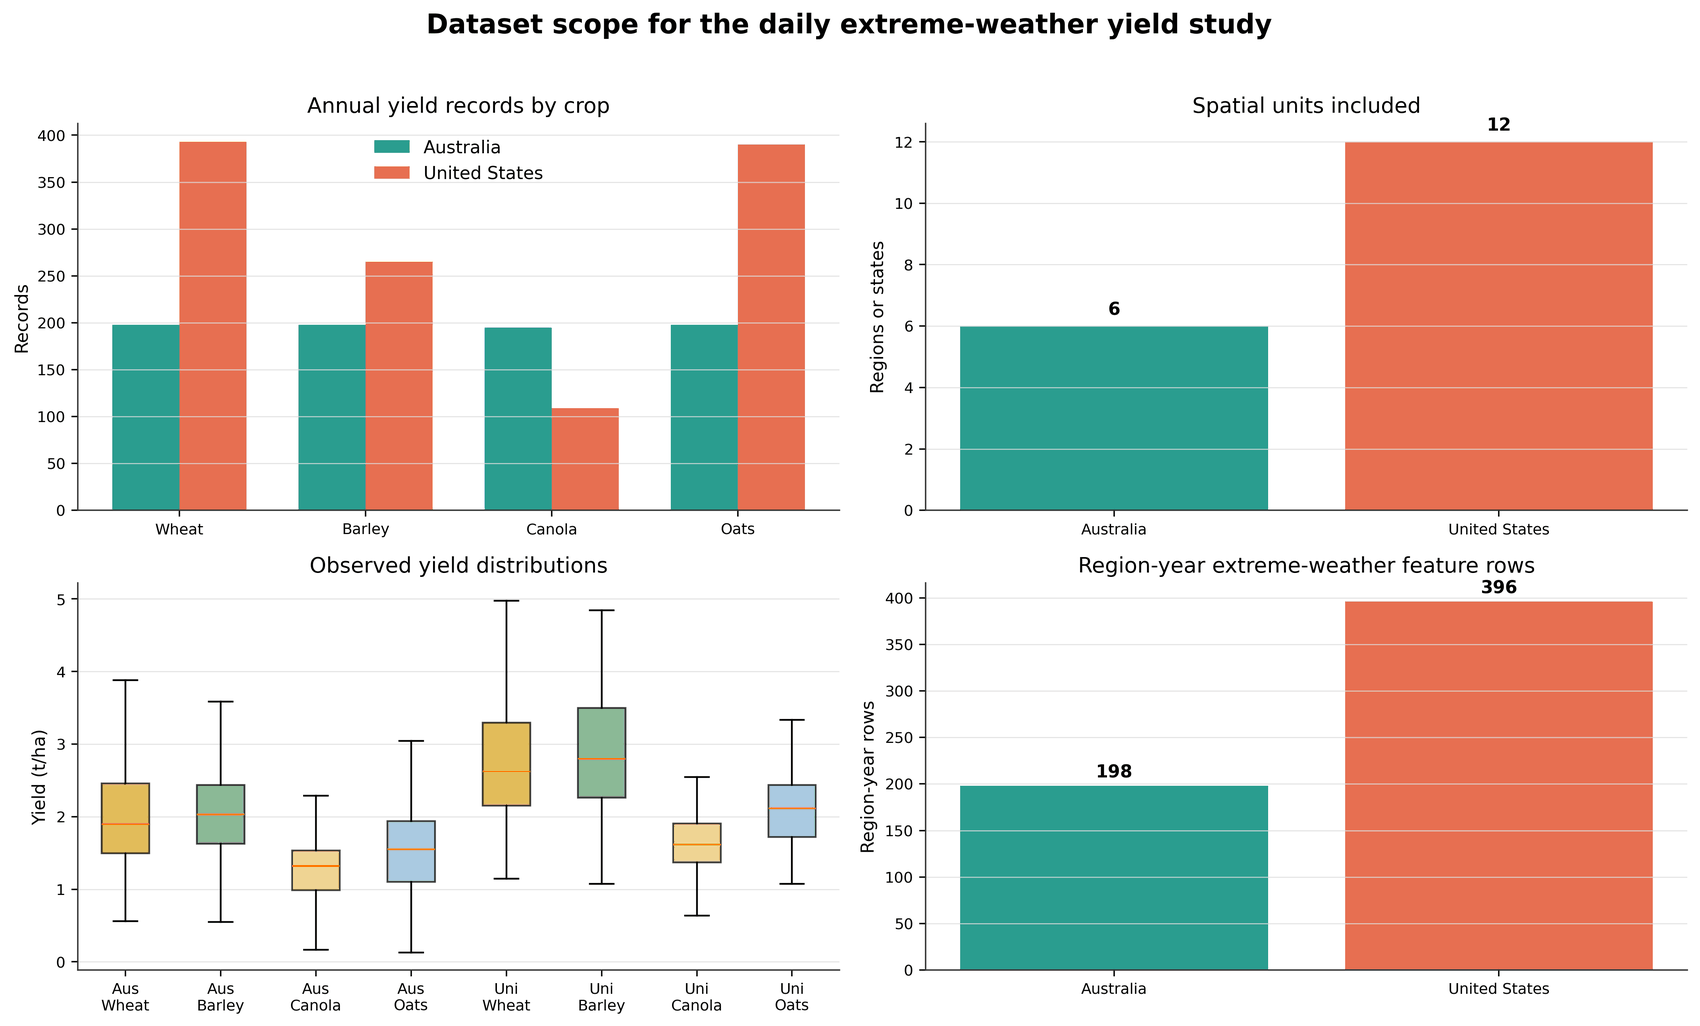
\includegraphics[width=0.92\textwidth,height=0.33\textheight,keepaspectratio]{figures/main/fig01_dataset_scope.png}
\caption{Dataset scope and modeling target. The figure summarizes the country, crop, region, yield, and region-year weather-feature coverage used to construct the crop-region-year modeling frame.}
\label{fig:dataset_scope}
\end{figure}

\section{Feature Engineering}
Daily weather records are aggregated into growing-season indicators using May--October as the common seasonal window. This is a harmonized proxy for comparing Australian and U.S. winter/overlap crops, not a crop-specific planting-to-harvest calendar; late-season rainfall indicators therefore summarize rainfall near the end of this proxy window rather than actual pre-harvest exposure for every crop-region. The feature set includes rainfall totals and means, dry-day counts, maximum dry-spell length, heavy-rain intensity indicators, heat-day counts, cold and frost exposure, growing degree days, and seasonal radiation summaries. This design is consistent with prior yield-prediction studies showing that weather and environmental inputs are central predictors in both classical machine-learning and deep-learning yield models \citep{vanKlompenburg2020CropYieldReview,Pathak2023InputModalities,Jabed2024Comprehensive}. These variables are intentionally interpretable so that model outputs can be explained in agronomic language.

Soil variables are added as persistent regional context. Weather features represent year-specific seasonal stress, while soil features represent slower-changing growing conditions. The main modeling comparison evaluates crop-region-year plus weather-feature sets with soil excluded and a corresponding weather-plus-soil setting, following the broader multi-source feature-design direction used in recent crop-yield modeling work \citep{Bansal2023WinterWheatHeterogeneous,Lu2024MultiSourceDL,Ashfaq2025DeepAgroNet}. The indicator groups are defined in Table~\ref{tab:feature_definitions}, and Figure~\ref{fig:feature_design} summarizes the feature-engineering workflow.

\begin{table}[H]
\centering
\caption{Grouped definitions of the daily extreme-weather indicators used to construct the crop-region-year model frame.}
\label{tab:feature_definitions}
\small
\setlength{\tabcolsep}{5pt}
\renewcommand{\arraystretch}{1.18}
\begingroup
\arrayrulecolor{black!55}
\begin{tabularx}{\textwidth}{p{0.22\textwidth}Yp{0.24\textwidth}}
\toprule
Indicator group & Computation / threshold & Output \\
\midrule
\arrayrulecolor{black!18}
Seasonal rainfall & Sum and mean of daily rainfall over May--Oct. & \texttt{rain\_sum}; \texttt{rain\_mean} \\
\hline
Radiation & Sum and mean of daily solar radiation over May--Oct. & \texttt{radiation\_sum}; \texttt{radiation\_mean} \\
\hline
Growing degree days & Sum of max($Tmean_d - 5^\circ$C, 0). If missing, $Tmean_d=(Tmax_d+Tmin_d)/2$. & degree-days \\
\hline
Seasonal windows & Repeat selected rainfall, dry, heat, frost, heavy-rain, and radiation features for early, mid, and late season. & early = May--Jun; mid = Jul--Aug; late = Sep--Oct \\
\hline
Dry exposure & Dry days use rain $<$ 1 mm and rain $<$ 2 mm. Dry spells are the longest consecutive dry run. Long dry-spell events count runs $\geq$ 7 or $\geq$ 14 days using rain $<$ 1 mm. & days; event count \\
\hline
Heavy-rain exposure & Count days with rain $\geq$ 10, 20, 25, or 50 mm/day. Also compute maximum rolling 1-, 3-, and 7-day rainfall. & days; mm \\
\hline
Heat exposure & Heat days use $Tmax_d \geq$ 30, 35, or 40$^\circ$C. Heatwave events count runs of at least 3 days at 30 or 35$^\circ$C. & days; event count \\
\hline
Heat degree days & Sum of max($Tmax_d - 30^\circ$C, 0) and max($Tmax_d - 35^\circ$C, 0). & $^\circ$C-days \\
\hline
Hot-dry days & Count days where $Tmax_d \geq$ 30$^\circ$C and rain $<$ 1 mm. & days \\
\hline
Frost and cold exposure & Frost days use $Tmin_d \leq$ 0$^\circ$C; cold days use $Tmin_d \leq$ 5$^\circ$C. Frost events require at least 2 consecutive frost days. & days; event count \\
\hline
Pre-harvest rain risk & Use the last 7, 14, and 21 days before Oct 31. Storm flag = 1 if last-21-day max 3-day rain $\geq$ 25 mm or last-14-day heavy-rain count $\geq$ 1. & mm; count; binary \\
\arrayrulecolor{black!55}
\bottomrule
\end{tabularx}
\arrayrulecolor{black}
\endgroup

\end{table}

\begin{figure}[!htbp]
\centering
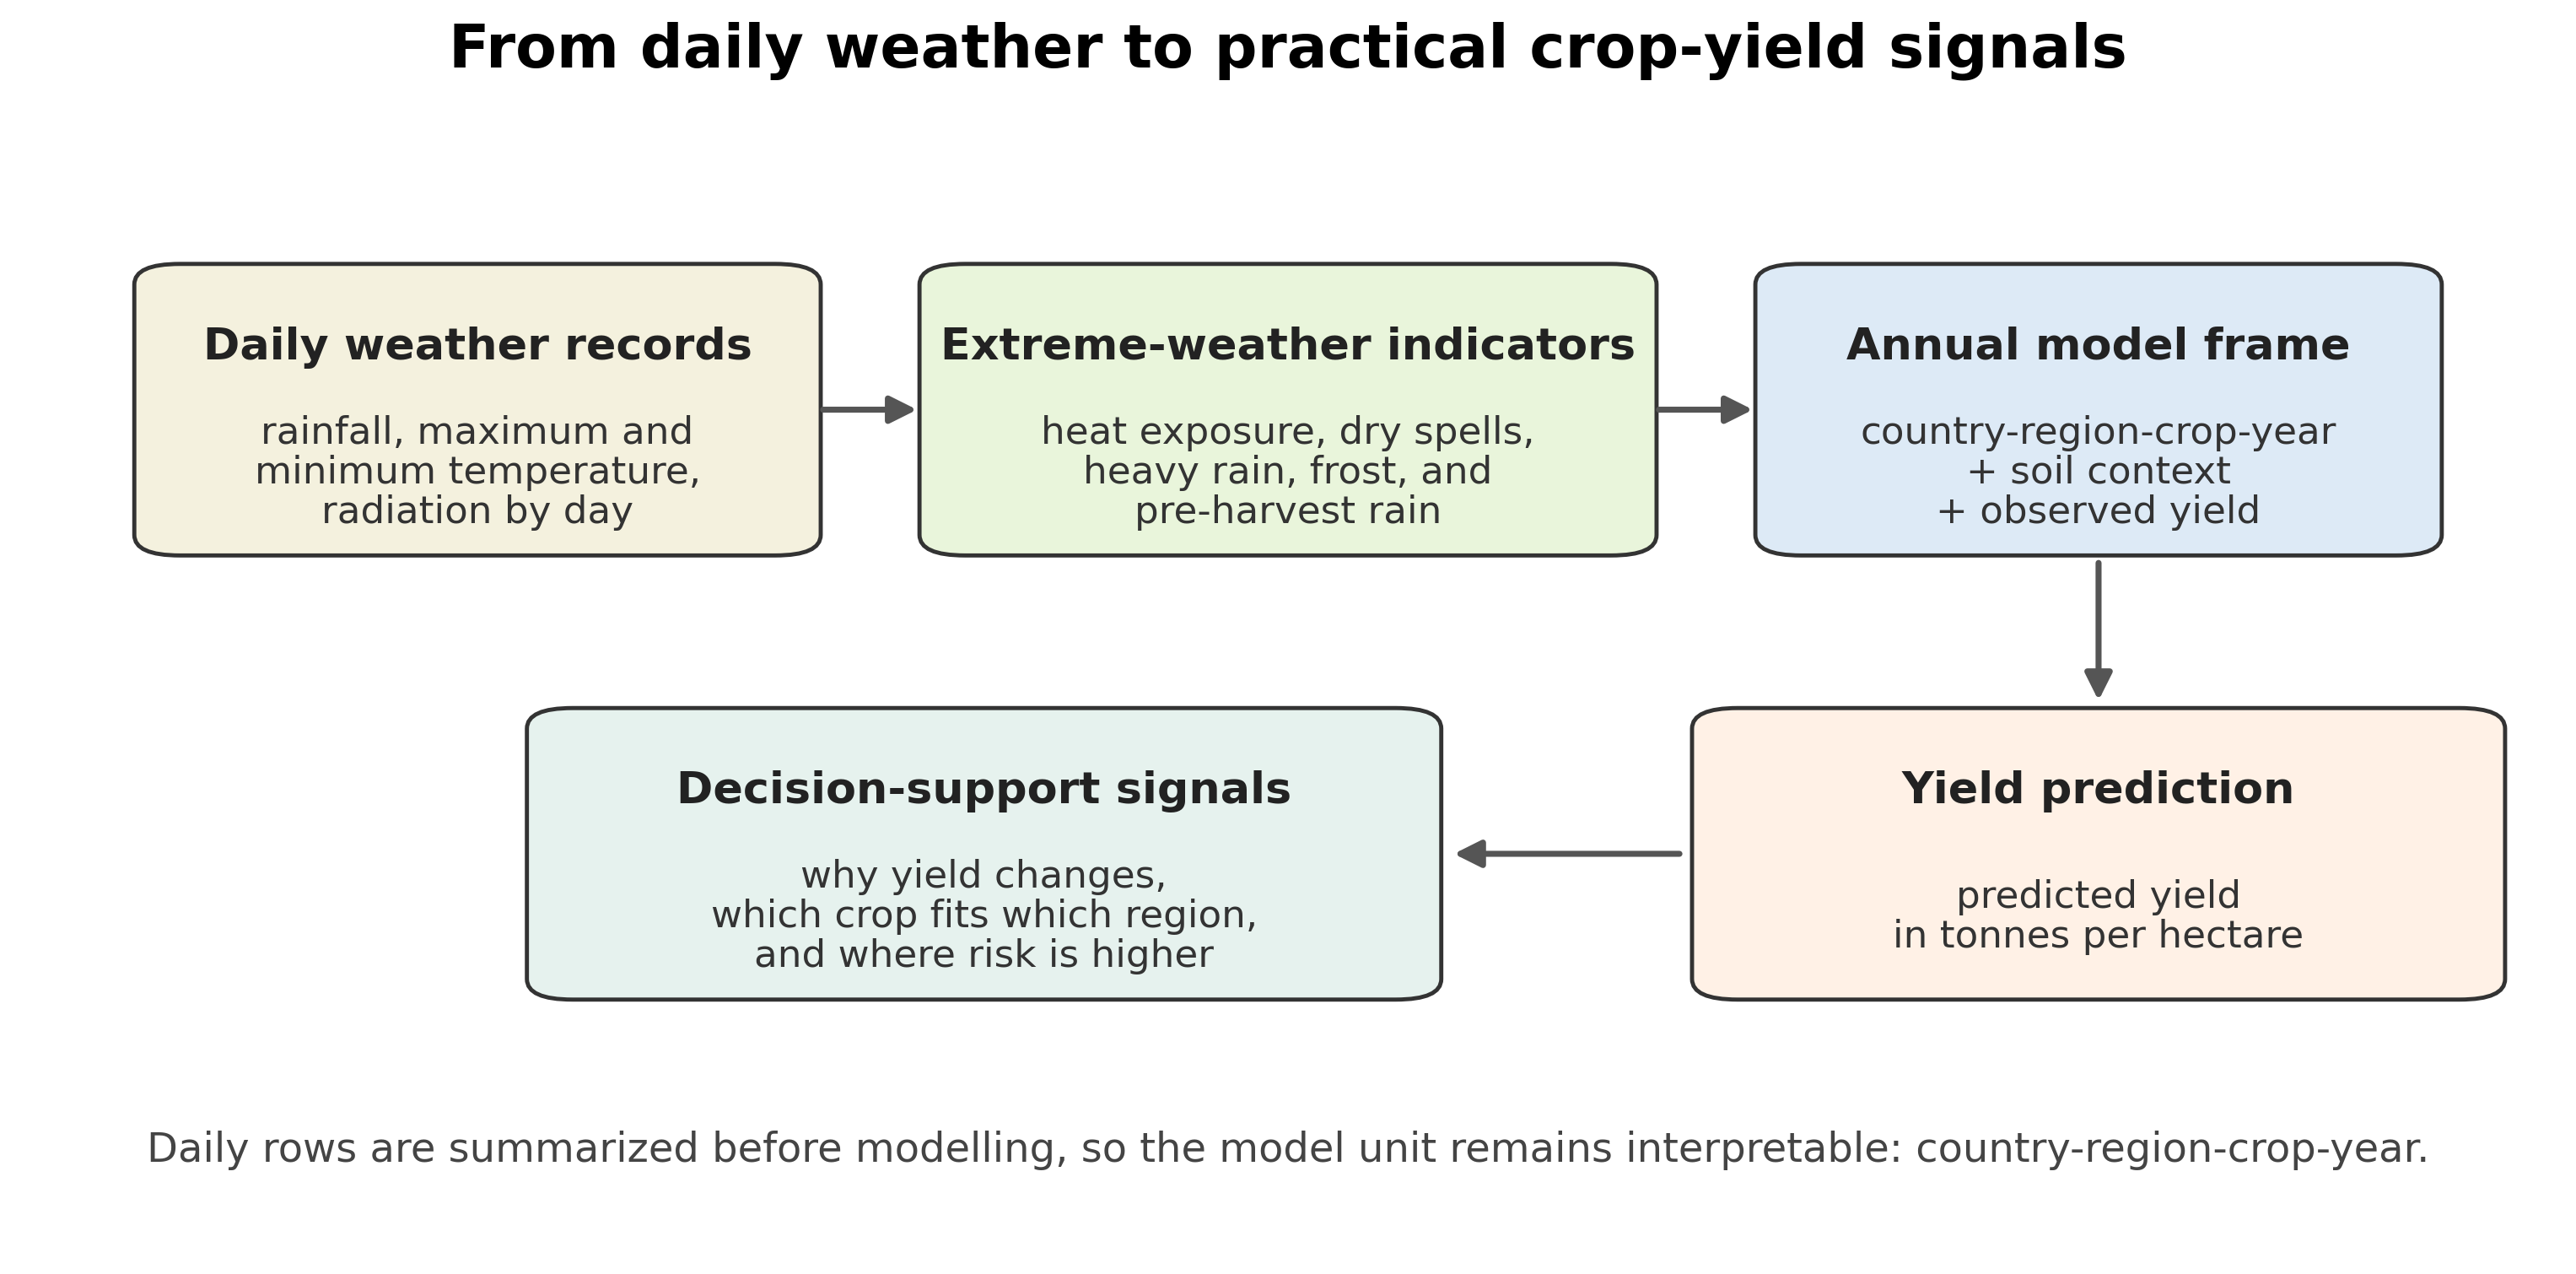
\includegraphics[width=0.92\textwidth,height=0.30\textheight,keepaspectratio]{figures/main/fig02_daily_extreme_feature_design.png}
\caption{Daily extreme-weather feature design. Daily weather observations are aggregated into interpretable growing-season indicators, merged with soil context, and used for yield prediction, crop-region suitability, and weather-conditioned crop comparison.}
\label{fig:feature_design}
\end{figure}

\section{Modeling Strategy}
The model set includes linear and nonlinear learners: Ridge regression, ElasticNet, Random Forest, Extra Trees, Histogram Gradient Boosting, and a multilayer perceptron neural network. Comparing multiple model families is useful because crop-yield studies often find that performance depends on the crop, region, feature set, and evaluation design rather than on one universally best algorithm \citep{Iniyan2023Techniques,Panigrahi2023Comparative,Jhajharia2023MLDL,Mahesh2024Gradient}. Learning-algorithm selection uses a forward-time validation protocol. Candidate algorithms are first trained on 1989--2010 and compared on 2011--2015 within each pre-specified modeling task. The selected learning algorithm is then refitted on 1989--2015 and evaluated once on the final 2016--2021 test period. This design better represents future-season prediction than a random split and avoids choosing the best model directly from the test set \citep{Morales2023PastFuture,Joshi2024TransferLearning}.

The model settings were fixed before final testing. Ridge used $\alpha=1.0$; ElasticNet used $\alpha=0.003$, $l1\_ratio=0.25$, and 10,000 maximum iterations. Random Forest used 250 trees with a minimum leaf size of 2, and Extra Trees used 350 trees with a minimum leaf size of 2. Histogram Gradient Boosting used 350 boosting iterations, a learning rate of 0.045, and $l2$ regularization of 0.05. The neural network used two hidden layers with 64 and 32 units, ReLU activation, $\alpha=0.001$, learning rate 0.001, up to 900 iterations, and early stopping with a 15\% internal validation fraction.

Model performance is evaluated with RMSE and R$^2$. RMSE is reported in tonnes per hectare. Two simple baselines are also evaluated for the combined overlap-crop task: a historical crop-region mean baseline and a previous-year yield baseline. The previous-year yield baseline is kept as an external persistence benchmark rather than a model input, because the decision-support model is intended to isolate weather-conditioned signals and to score candidate crops for which a crop-specific lagged yield may not be available. Feature-group ablation compares crop-region-year only, crop-region-year plus rainfall features, crop-region-year plus temperature features, crop-region-year plus radiation features, crop-region-year plus extreme-event features, all weather features excluding soil, and weather-plus-soil feature sets. Interpretation is based on feature-group ablation, high-versus-low yield comparisons, and weather-conditioned crop rankings. This emphasis on post-model interpretation follows recent explainable-AI work warning that black-box yield models require careful, domain-aware explanation before being used for climate or planning conclusions \citep{Hu2023ExplainableYield,Mohan2025AIXAI}.

For weather-conditioned crop suitability, candidate crops are interpreted as model-based screening alternatives rather than direct planting recommendations. This crop-choice step uses the main crop-region-year plus extreme-weather model, with the learning algorithm selected on the validation period and soil variables excluded from the counterfactual crop-ranking step, while still retaining crop, country, region, and year identifiers used by the prediction pipeline. Crop comparisons are strongest when both the best crop and the runner-up have historical records in the same region. The reported crop-choice table is therefore filtered to region-observed candidate crops. These rankings do not account for cultivar choice, planting calendar, irrigation, fertilizer, disease pressure, input cost, or market constraints. Table~\ref{tab:best_models} reports the algorithm selected for each pre-specified modeling task, and Table~\ref{tab:feature_group_ablation} reports validation and final-test metrics for the diagnostic baseline and feature-group ablation.

\begin{table}[H]
\centering
\caption{Learning algorithm selected for each pre-specified modeling task. For each task, the learning algorithm is selected on 2011--2015 validation performance, refitted on 1989--2015, and reported on the 2016--2021 test period.}
\label{tab:best_models}
\scriptsize
\resizebox{\textwidth}{!}{\begin{tabular}{llllrrr}
\toprule
Dataset & Feature set & Selected model & Validation R$^2$ & Test R$^2$ & Test RMSE & Test rows \\
\midrule
Australia + U.S. overlap crops & Extreme-weather only & ExtraTrees & 0.777 & 0.718 & 0.661 & 353 \\
Australia + U.S. wheat & Extreme-weather only & ElasticNet & 0.667 & 0.689 & 0.697 & 105 \\
Australia overlap crops & Extreme-weather + soil & HistGradientBoosting & 0.602 & 0.490 & 0.890 & 144 \\
U.S. overlap crops & Extreme-weather only & ExtraTrees & 0.851 & 0.801 & 0.534 & 209 \\
\bottomrule
\end{tabular}
}
\end{table}

\begin{table}[H]
\centering
\caption{Diagnostic baseline and feature-group ablation for the combined Australia and U.S. overlap-crop task. Feature-group rows retain crop, country, region, and year identifiers unless they are explicit baselines; named weather groups add the stated weather features and exclude soil except in the weather-plus-soil row. Within each row, the learning algorithm is selected by validation performance, then refitted and evaluated on the 2016--2021 test period.}
\label{tab:feature_group_ablation}
\scriptsize
\setlength{\tabcolsep}{3pt}
\renewcommand{\arraystretch}{1.08}
\input{tables/table03_weather_vs_weather_soil.tex}
\end{table}

\section{Results}
\subsection{Predictive Performance}
The validation-based time-split evaluation shows that daily extreme-weather indicators contain useful information for crop-yield prediction, but it also shows that simple crop-region temporal baselines are strong. In the combined Australia and U.S. overlap-crop task, the main crop-region-year plus extreme-weather model, with the learning algorithm selected on the validation period and soil variables excluded, used ExtraTrees and reached a test RMSE of 0.661 t/ha and a test R$^2$ of 0.718. This performance was competitive with, but slightly below, the previous-year yield baseline on the final test set. The U.S. overlap-crop model achieved the strongest held-out performance, with ExtraTrees reaching a test RMSE of 0.534 t/ha and a test R$^2$ of 0.801. The Australia-only overlap-crop task was more difficult, with Histogram Gradient Boosting selected on validation and obtaining a test R$^2$ of 0.490. For the cross-country wheat-only task, the selected algorithm was ElasticNet, with a test RMSE of 0.697 t/ha and a test R$^2$ of 0.689.

The ablation results clarify where the predictive signal comes from. For the combined overlap-crop task, the historical crop-region mean baseline achieved a test R$^2$ of 0.604, and the previous-year yield baseline achieved a test R$^2$ of 0.720. Among weather groups, crop-region-year plus temperature features and crop-region-year plus rainfall features reached test R$^2$ values of 0.751 and 0.746, respectively. The weather-plus-soil setting reached a test R$^2$ of 0.729. These results suggest that daily weather features are informative, especially temperature and rainfall summaries, but that crop-region history and temporal persistence remain important benchmarks. The main value of the weather-feature workflow is therefore not simply beating a persistence baseline, but providing interpretable planning signals about weather-conditioned yield risk and crop suitability. The feature-group ablation in Table~\ref{tab:feature_group_ablation} is used diagnostically to understand predictive signal, not to replace the pre-specified all-weather decision-support model. Therefore, Table~\ref{tab:feature_group_ablation} reports validation RMSE/R$^2$ and final-test RMSE/R$^2$ side by side, while the final test-period ablation is not used for post-hoc model selection. Figure~\ref{fig:model_performance} summarizes the time-split performance, and Figure~\ref{fig:actual_predicted} compares observed and predicted test yields.

Permutation importance was computed for the main Australia and U.S. overlap-crop model on the final 2016--2021 test period. The strongest overall predictors included crop and region identifiers as well as geographic coordinates such as \texttt{lat\_mean} and \texttt{lon\_mean}, confirming that crop-region structure and location-specific climate context influence predictions. Figure~\ref{fig:feature_importance} reports the weather-feature subset of the permutation ranking: radiation summaries, heat-day exposure, mean maximum temperature, seasonal rainfall, cold-day exposure, maximum consecutive heat days, and hot-dry days. The magnitudes are small in RMSE units, so the ranking is used as an interpretability aid rather than as evidence of causal weather effects. The permutation analysis is used only for post-hoc interpretation of the held-out predictions and is not used for model selection.

\begin{figure}[!htbp]
\centering
\captionsetup{font=small,skip=3pt}
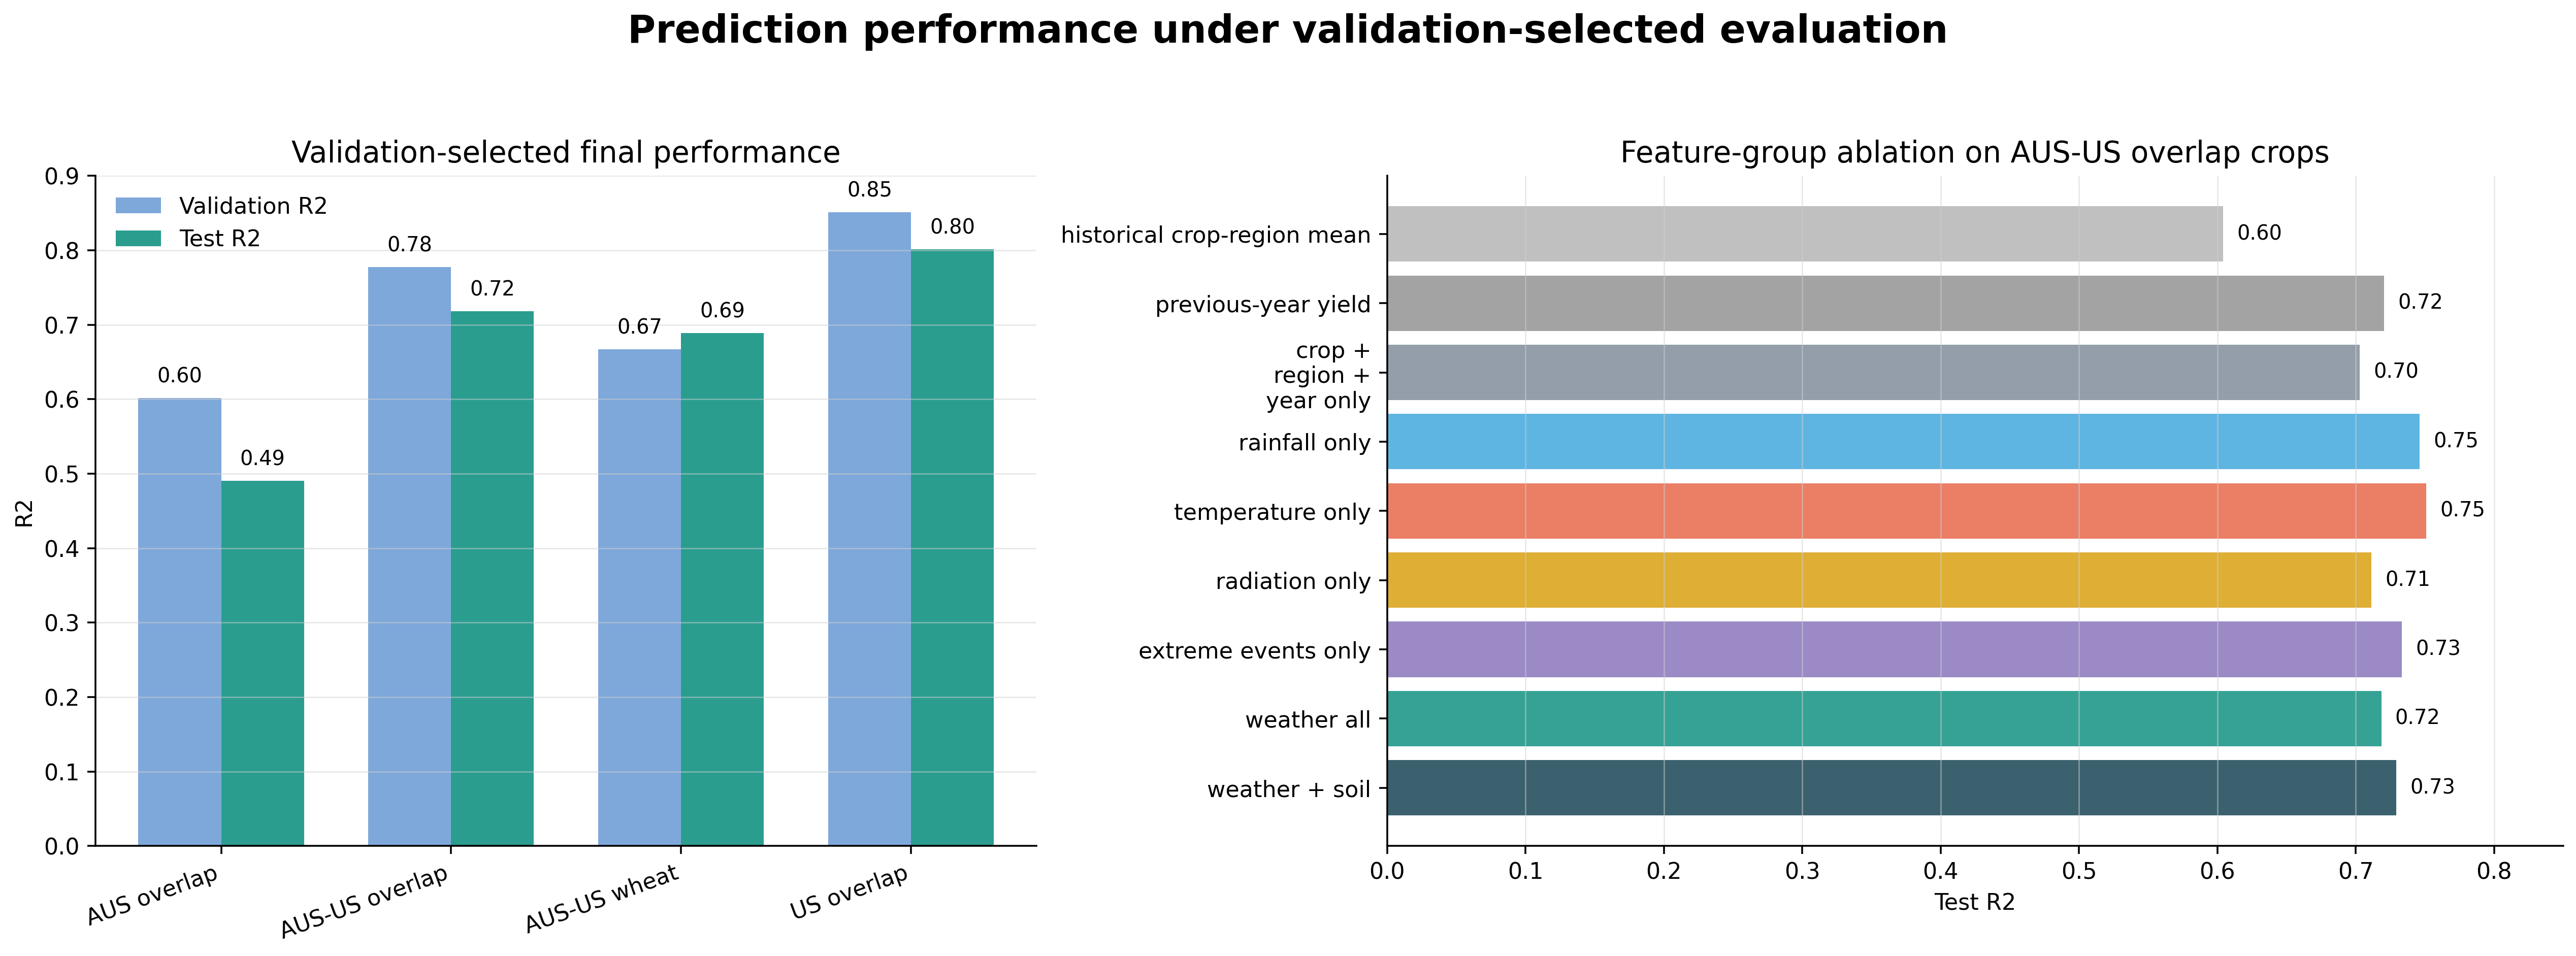
\includegraphics[width=0.84\textwidth,height=0.22\textheight,keepaspectratio]{figures/main/fig03_model_performance.png}
\caption{Time-split model performance and feature-group ablation. Bars report validation and test R$^2$ values for the selected learning algorithm in each pre-specified task, and the ablation panel reports test R$^2$ for baseline and feature-group settings in the combined Australia and U.S. overlap-crop task.}
\label{fig:model_performance}

\vspace{0.35em}

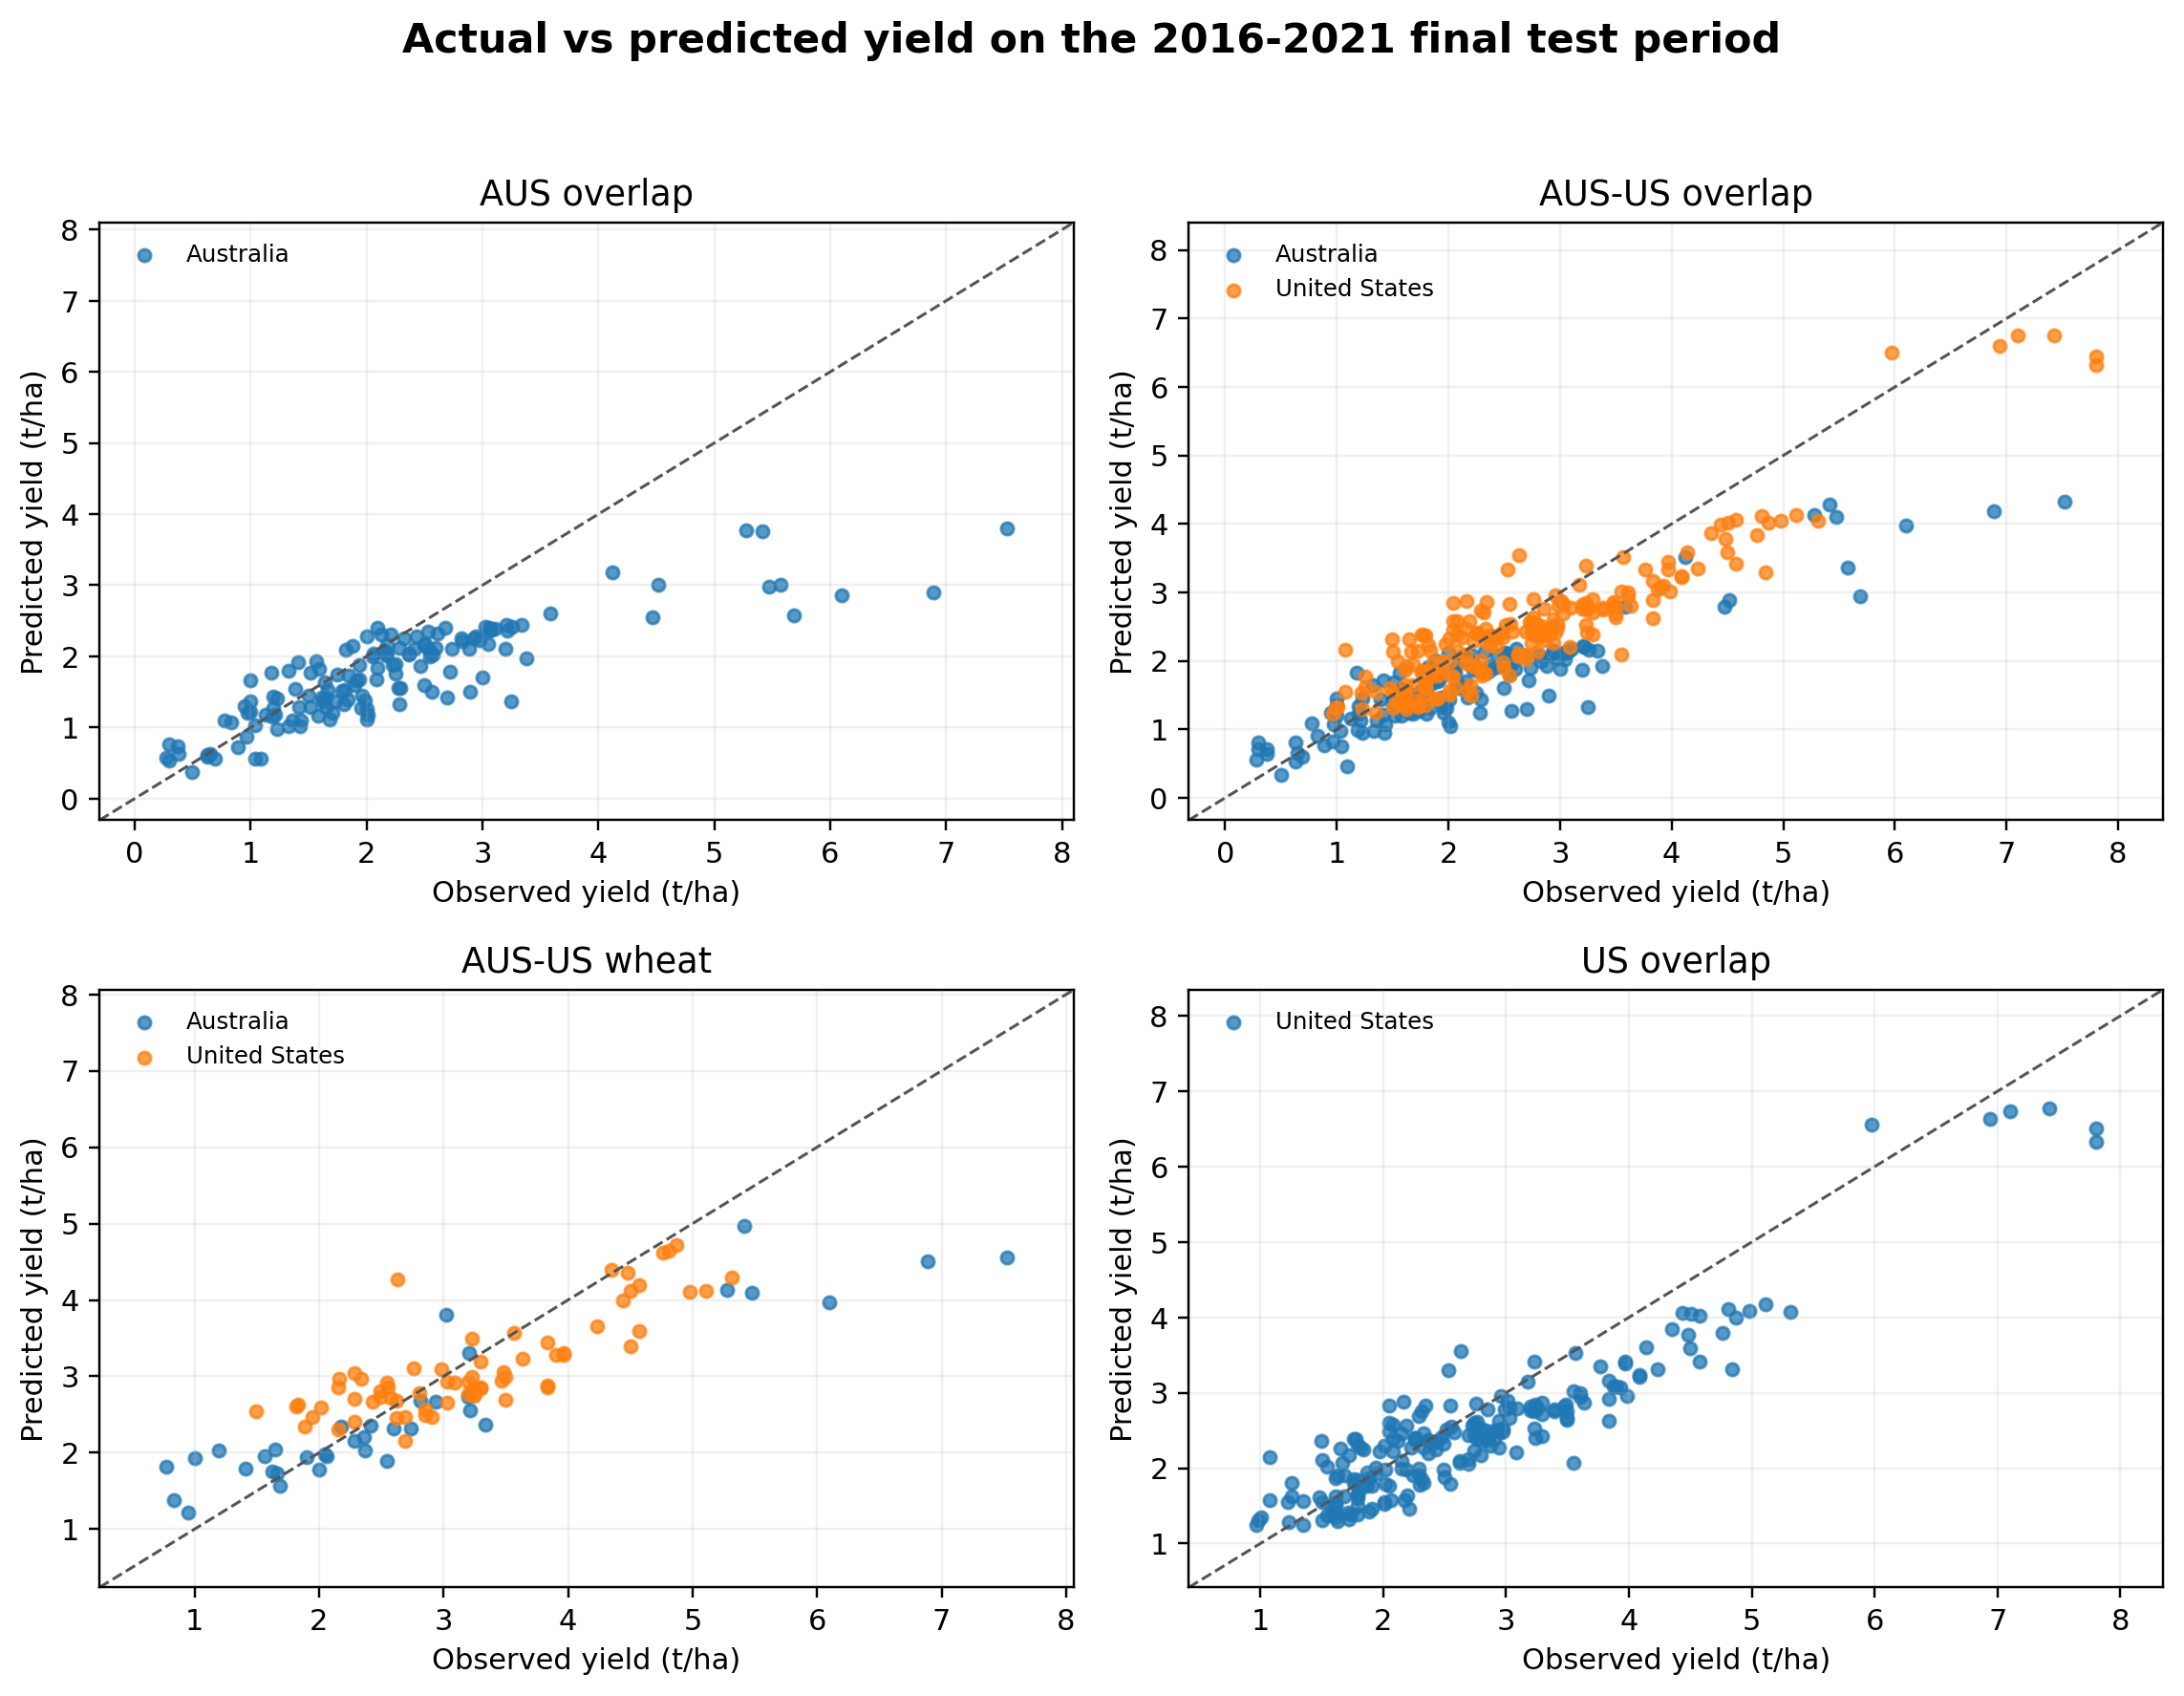
\includegraphics[width=0.80\textwidth,height=0.40\textheight,keepaspectratio]{figures/main/fig04_actual_vs_predicted_test.png}
\caption{Observed versus predicted yield in the held-out test period. Each point represents a crop-region-year observation in 2016--2021, allowing visual assessment of model calibration in the original yield scale.}
\label{fig:actual_predicted}
\end{figure}

\begin{figure}[!htbp]
\centering
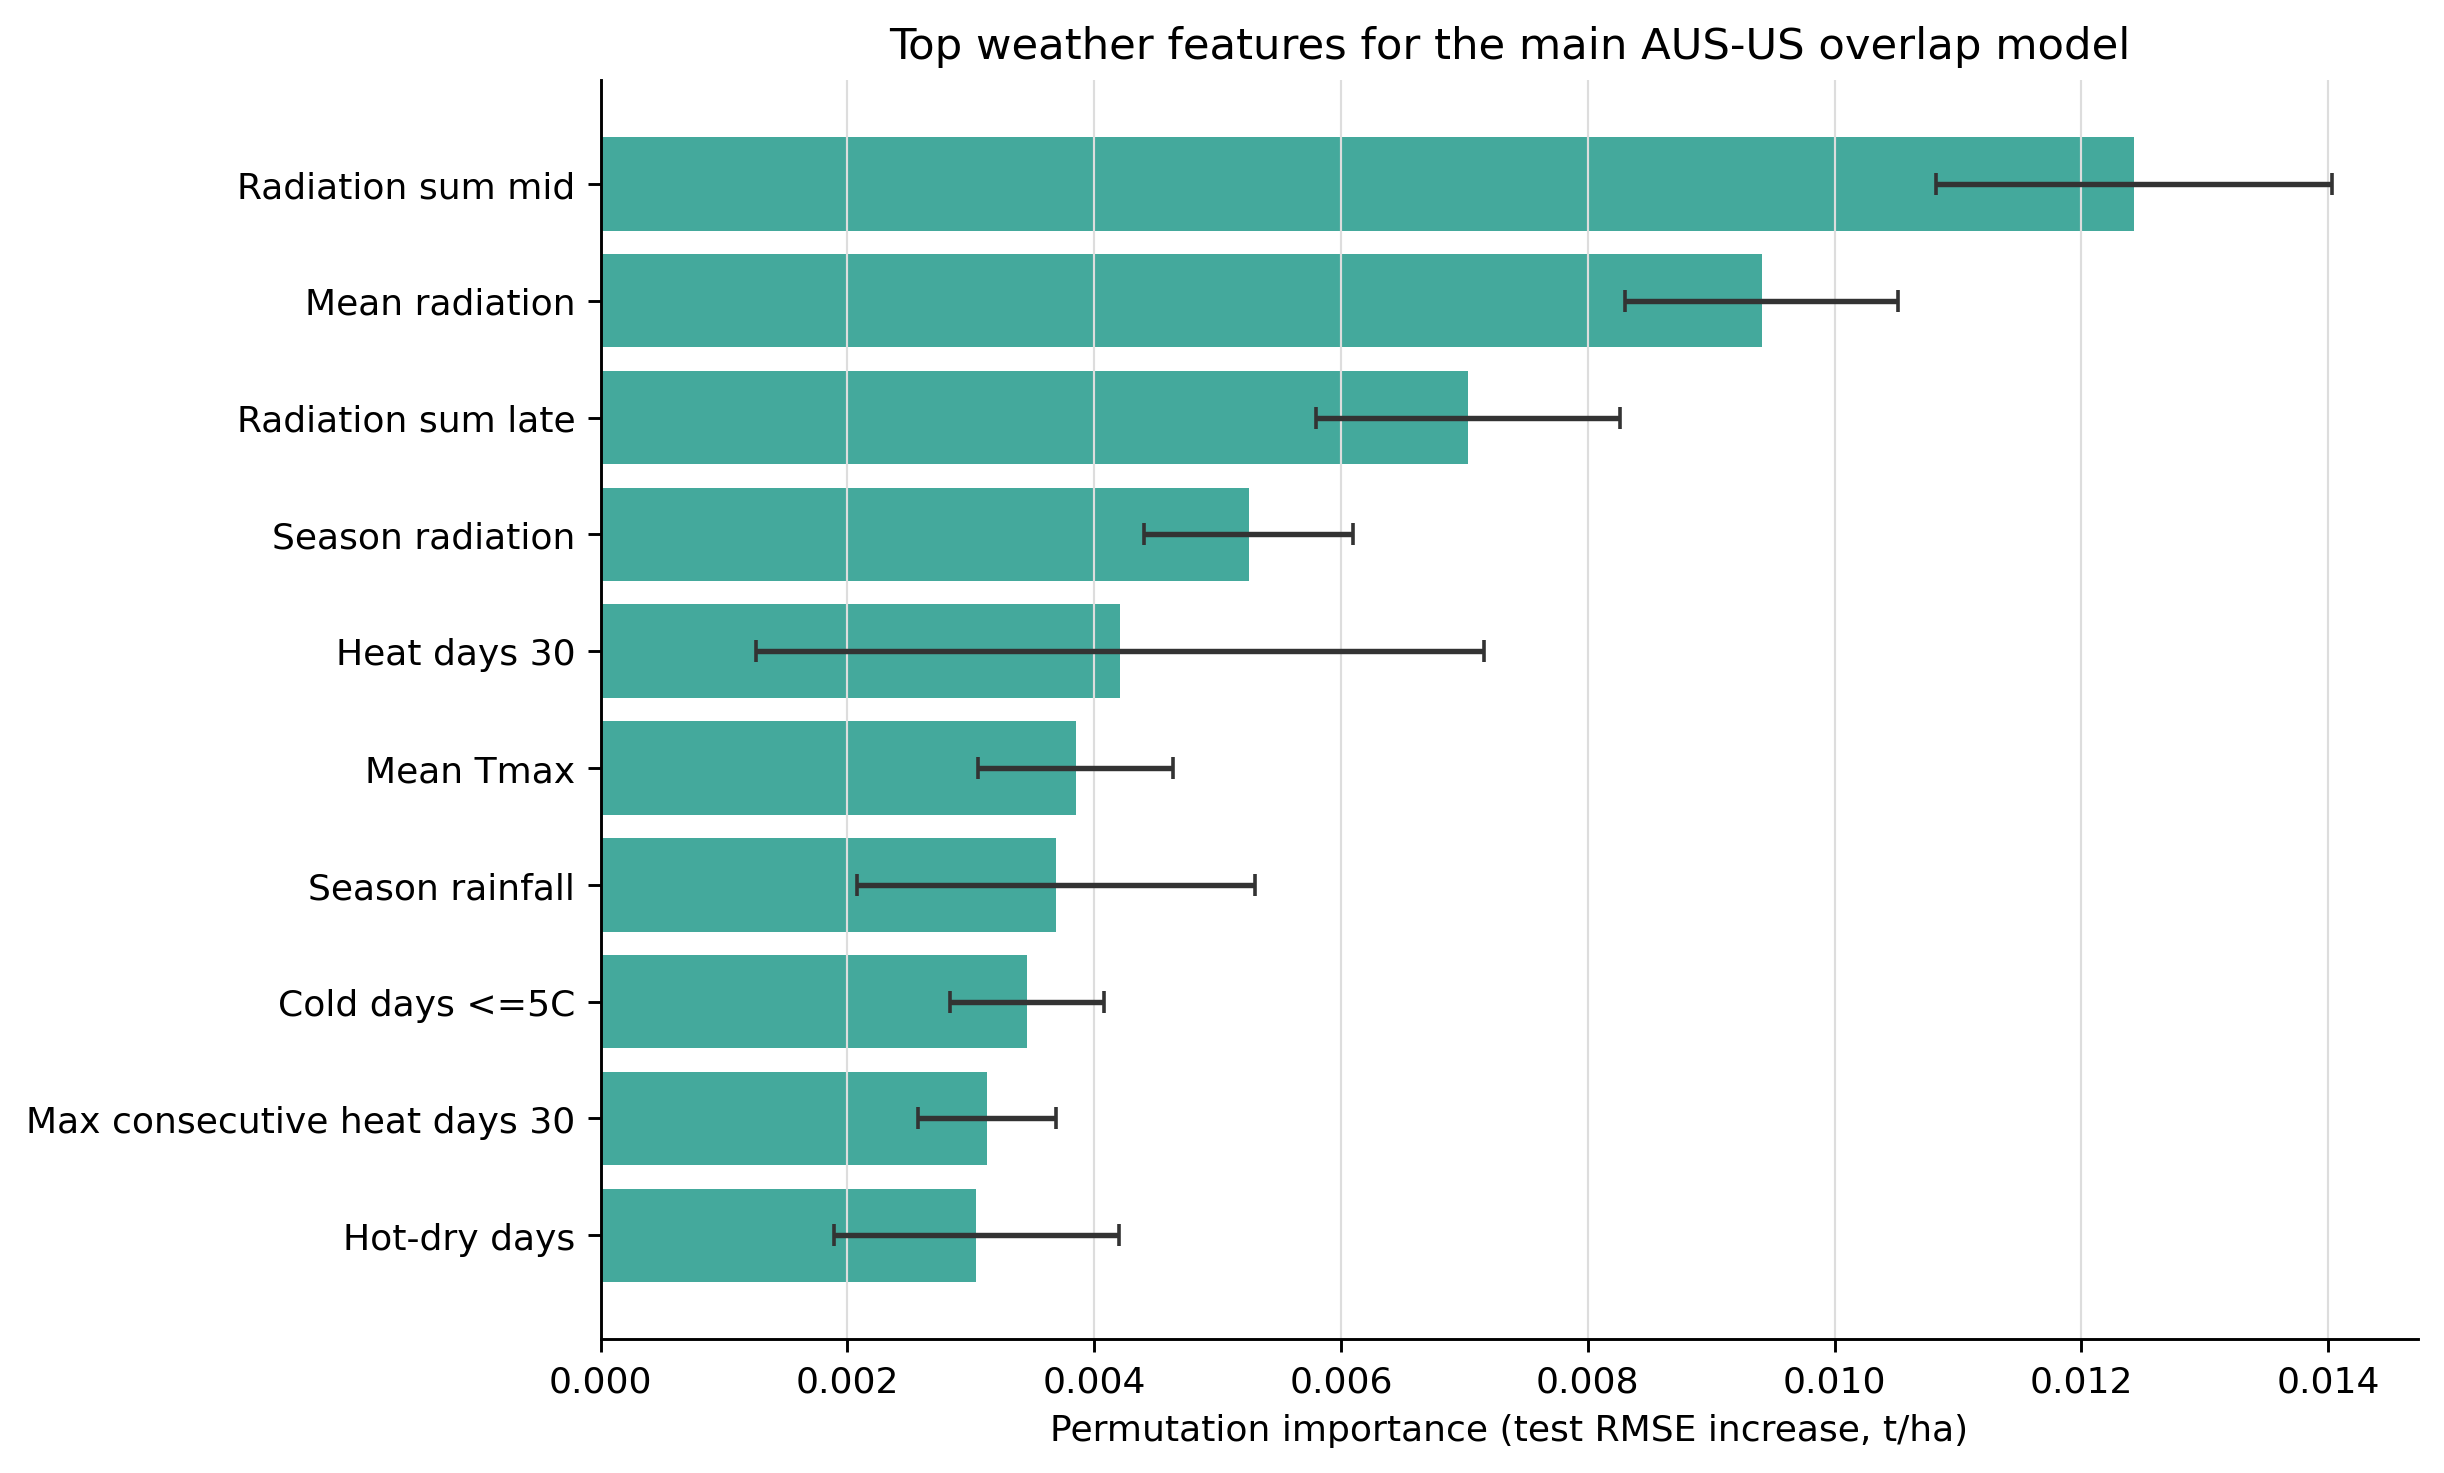
\includegraphics[width=0.88\textwidth]{figures/main/fig05_top_feature_importance.png}
\caption{Permutation importance of the top weather features for the main combined Australia and U.S. overlap-crop model. The full permutation ranking is interpreted together with crop, region, and geographic-coordinate predictors; this panel shows the weather-feature subset for readability. Values show the mean increase in test RMSE when a feature is permuted, with error bars showing one standard deviation over 20 repeats.}
\label{fig:feature_importance}
\end{figure}

\subsection{Crop-Region Yield Change}
Observed yield changes were crop-specific and region-specific. The largest observed gain occurred for Australia Tasmania Wheat, where mean yield increased by 1.986 t/ha from 1989--2000 to 2010--2021. The next largest gain was United States Colorado Barley, with an increase of 1.923 t/ha. The largest observed decreases were Australia New South Wales Oats, which declined by 0.350 t/ha, and United States Washington Oats, which declined by 0.270 t/ha. Table~\ref{tab:yield_gain_loss} lists selected yield gains and losses, and Figure~\ref{fig:yield_change} maps the observed yield changes.

\begin{table}[H]
\centering
\caption{Selected crop-region yield gains and losses between early and recent periods.}
\label{tab:yield_gain_loss}
\scriptsize
\resizebox{\textwidth}{!}{\begin{tabular}{lllllll}
\hline
country & region & crop & early yield, 1989-2000 & recent yield, 2010-2021 & change, t/ha & status \\
\hline
Australia & Tasmania & Wheat & 3.535 & 5.522 & 1.986 & increase \\
United States & Colorado & Barley & 5.107 & 7.030 & 1.923 & increase \\
Australia & Tasmania & Barley & 2.559 & 4.066 & 1.507 & increase \\
United States & Minnesota & Wheat & 2.587 & 3.767 & 1.179 & increase \\
United States & Illinois & Wheat & 3.396 & 4.545 & 1.149 & increase \\
Australia & Tasmania & Canola & 1.125 & 2.174 & 1.049 & increase \\
United States & Iowa & Wheat & 2.707 & 3.609 & 0.902 & increase \\
United States & North Dakota & Wheat & 2.075 & 2.882 & 0.807 & increase \\
Australia & New South Wales & Oats & 1.464 & 1.114 & -0.350 & decrease \\
United States & Washington & Oats & 2.526 & 2.256 & -0.270 & decrease \\
United States & South Dakota & Barley & 2.385 & 2.222 & -0.163 & stable \\
Australia & New South Wales & Canola & 1.525 & 1.446 & -0.079 & stable \\
Australia & Queensland & Oats & 0.684 & 0.639 & -0.045 & stable \\
United States & Montana & Oats & 1.835 & 1.805 & -0.030 & stable \\
\hline
\end{tabular}
}
\end{table}

\begin{figure}[H]
\centering
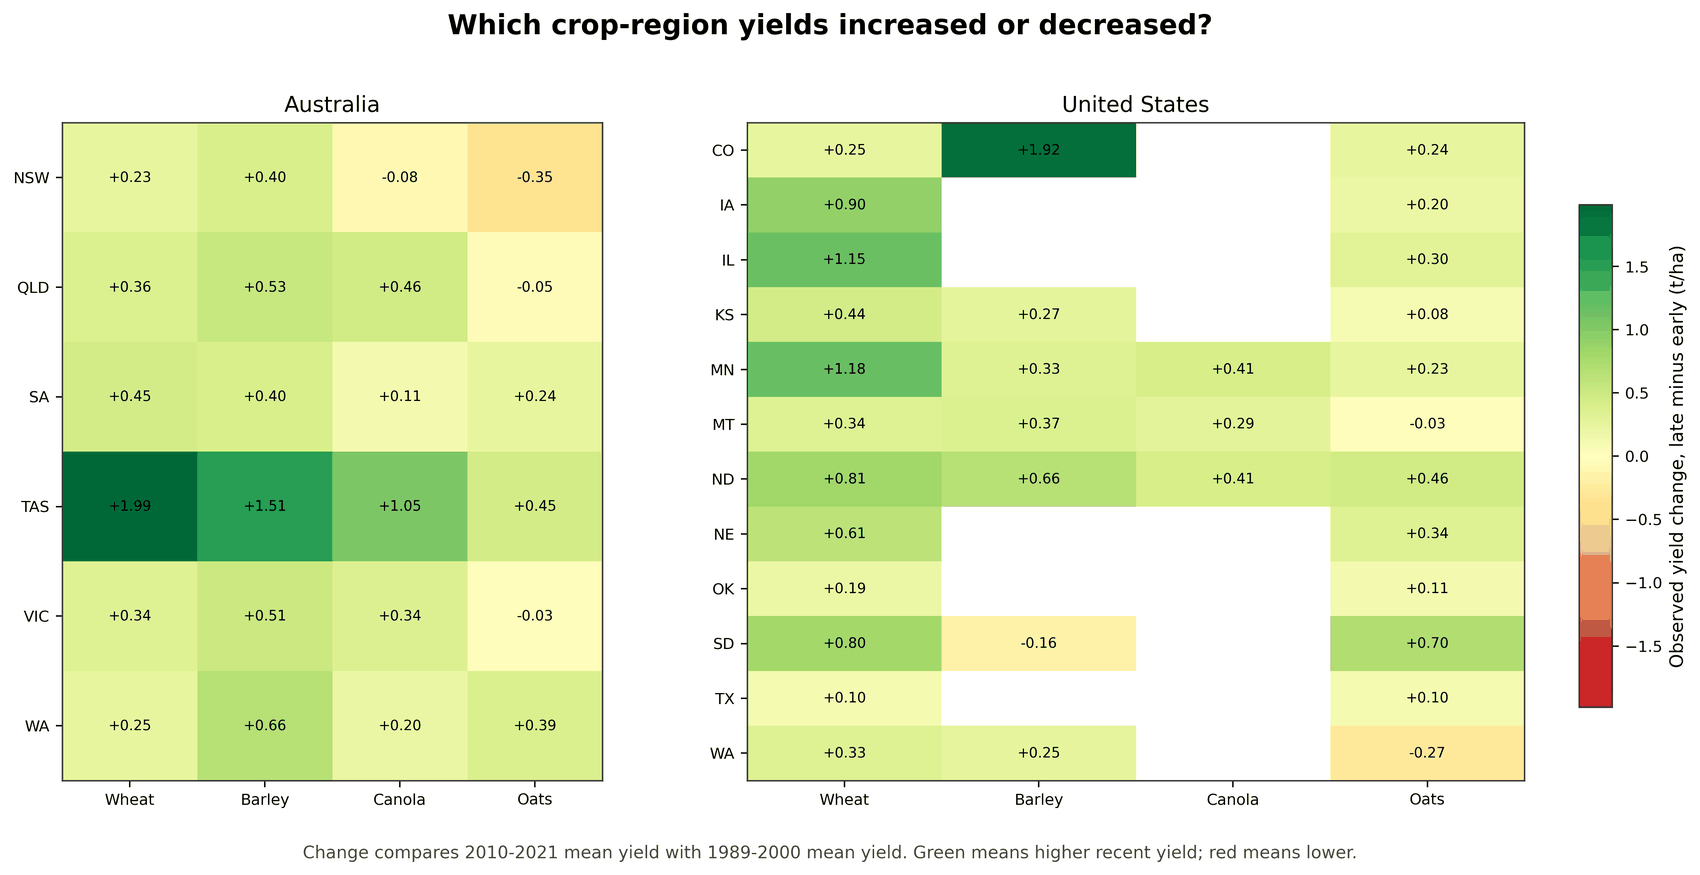
\includegraphics[width=\textwidth]{figures/main/fig17_observed_yield_change_region_crop.png}
\caption{Observed yield change by crop and region. The heatmap compares mean yield in 1989--2000 with mean yield in 2010--2021, identifying crop-region combinations with the largest increases or decreases.}
\label{fig:yield_change}
\end{figure}

\subsection{Weather Signatures of High-Yield Years}
The high-versus-low yield comparison translates model results into weather language. For each crop-region pair, the analysis compares the highest predicted-yield years with the lowest predicted-yield years and records which weather indicators differ most. This comparison is used as an interpretability layer rather than as causal attribution, consistent with cautions in explainable yield modeling \citep{Hu2023ExplainableYield,Morales2023PastFuture}. The strongest high-low gap was found for United States Colorado Barley, where the predicted difference between high-yield and low-yield years was 1.667 t/ha. High-yield years in that crop-region pair were associated with higher mean minimum temperature, higher growing degree days, higher mean maximum temperature, and a longer dry spell.

A second strong example was Australia New South Wales Wheat, with a predicted high-low gap of 1.624 t/ha. High-yield years were associated with higher seasonal rainfall, higher daily rainfall, higher maximum three-day rainfall, and lower seasonal radiation. These statements should be interpreted as predictive associations within the dataset, not causal effects. Table~\ref{tab:weather_stories} and Figure~\ref{fig:weather_signatures} summarize these high-versus-low weather signatures.

\begin{table}[!htbp]
\centering
\caption{Weather signatures separating high-predicted-yield years from low-predicted-yield years. The gap is the predicted yield difference within each crop-region pair.}
\label{tab:weather_stories}
\footnotesize
\setlength{\tabcolsep}{3pt}
\renewcommand{\arraystretch}{1.15}
\begin{tabularx}{\textwidth}{p{0.12\textwidth}p{0.15\textwidth}p{0.08\textwidth}p{0.08\textwidth}Y}
\toprule
Country & Region & Crop & Gap & Weather indicators in high-yield years \\
\midrule
United States & Colorado & Barley & 1.667 & Higher mean minimum temperature (+0.6 C), higher growing degree days (+114.3 degree-days), higher mean maximum temperature (+0.7 C), and longer dry spell (+4.1 days). \\
Australia & New South Wales & Wheat & 1.624 & Higher seasonal rainfall (+255.1 mm), higher daily rainfall (+1.4 mm/day), higher maximum 3-day rainfall (+27.8 mm), and lower seasonal radiation (-185.1 MJ/m2). \\
Australia & New South Wales & Barley & 1.492 & Higher daily rainfall (+1.1 mm/day), higher seasonal rainfall (+194.7 mm), lower late-season radiation (-113.4 MJ/m2), and lower seasonal radiation (-167.7 MJ/m2). \\
Australia & Tasmania & Wheat & 1.420 & Lower late-season radiation (-56.8 MJ/m2), lower seasonal radiation (-80.7 MJ/m2), higher growing degree days (+70.3 degree-days), and higher mean maximum temperature (+0.4 C). \\
Australia & Victoria & Wheat & 1.389 & Higher seasonal rainfall (+163.6 mm), higher daily rainfall (+0.9 mm/day), more late-season rainfall (+29.0 mm), and higher maximum 3-day rainfall (+24.7 mm). \\
Australia & Victoria & Barley & 1.334 & Lower late-season radiation (-97.9 MJ/m2), fewer hot-dry days (-3.7 days), higher seasonal rainfall (+122.7 mm), and higher daily rainfall (+0.7 mm/day). \\
\bottomrule
\end{tabularx}

\end{table}

\begin{figure}[!htbp]
\centering
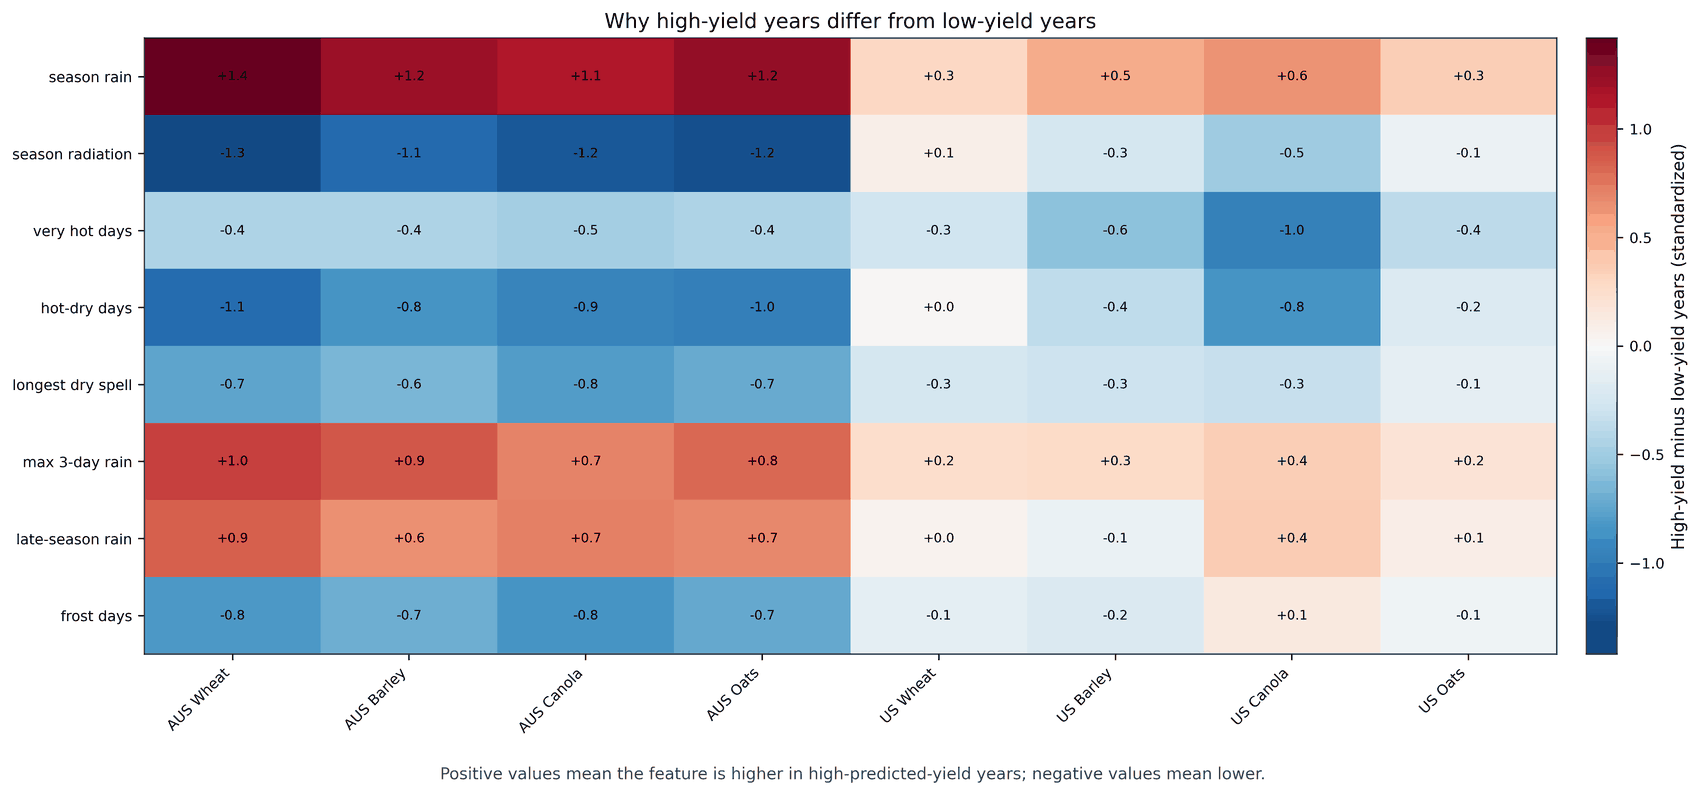
\includegraphics[width=\textwidth]{figures/main/fig19_high_vs_low_yield_weather_driver_matrix.png}
\caption{Weather signatures of high-yield years. For selected crop-region pairs, the figure compares weather indicators in high-predicted-yield years with low-predicted-yield years. Values should be interpreted as predictive associations rather than causal effects.}
\label{fig:weather_signatures}
\end{figure}

\subsection{Weather-Conditioned Crop Suitability}
The crop-choice analysis asks which crop is predicted to perform best under the same observed region-year weather profile using the main crop-region-year plus extreme-weather model, with the learning algorithm selected on the validation period and soil variables excluded from the counterfactual crop-ranking step. This turns yield prediction into a more practical planning signal and aligns with recent work framing yield modeling as a decision-support problem rather than only an accuracy benchmark \citep{Paudel2021LargeScaleForecasting,Pathak2023InputModalities,Jabed2024Comprehensive}. To reduce unsupported extrapolation, the reported crop-choice table uses candidate crops with historical records in the same region. Bootstrap intervals are added to indicate whether the largest crop-choice contrasts are stable under resampling of the 1989--2015 training-validation frame. These intervals reflect model resampling uncertainty only and do not include uncertainty from weather products, management, cultivar choice, irrigation, markets, or other unobserved constraints. The largest region-filtered crop-choice advantage occurred in United States Colorado in 2013, a cold/frost-stress year. Under that observed profile, Barley was predicted to outperform Oats by 4.809 t/ha, with a 95\% bootstrap interval of [3.90, 5.08] t/ha. Other strong cases included Australia Tasmania in 2014, where Wheat was predicted to outperform Barley by 2.066 t/ha with a 95\% interval of [0.66, 2.34] t/ha, and United States Illinois in 2013, where Wheat was predicted to outperform Oats by 2.000 t/ha with a 95\% interval of [1.11, 2.03] t/ha. Table~\ref{tab:crop_choice} reports the largest crop-choice advantages, while Figure~\ref{fig:suitability_map} and Figure~\ref{fig:crop_choice_advantage} show the spatial suitability and crop-choice advantage patterns.

\begin{table}[H]
\centering
\caption{Largest weather-conditioned crop-choice advantages under observed region-year weather profiles. Candidate crops are restricted to crops with historical records in the same region, and at most one case is shown per region. The 95\% CI is based on 120 bootstrap resamples of the 1989--2015 training-validation frame.}
\label{tab:crop_choice}
\scriptsize
\resizebox{\textwidth}{!}{\begin{tabular}{llllllllll}
\hline
country & region & year & weather regime & best crop & runner-up crop & advantage, t/ha & 95\% CI, t/ha & best yield, t/ha & candidates \\
\hline
United States & Colorado & 2013 & Cold/frost stress & Barley & Oats & 4.809 & [3.90, 5.08] & 7.130 & 3 \\
Australia & Tasmania & 2014 & Wet/storm risk & Wheat & Barley & 2.066 & [0.66, 2.34] & 5.257 & 4 \\
United States & Illinois & 2013 & Wet/storm risk & Wheat & Oats & 2.000 & [1.11, 2.03] & 4.474 & 2 \\
United States & Iowa & 2006 & Moderate season & Wheat & Oats & 1.437 & [0.48, 1.86] & 4.160 & 2 \\
United States & Washington & 2003 & Dry-spell stress & Wheat & Barley & 1.383 & [0.46, 1.47] & 3.958 & 4 \\
United States & Kansas & 1998 & Hot-dry stress & Wheat & Barley & 1.216 & [0.22, 1.39] & 3.126 & 4 \\
United States & Minnesota & 1993 & Moderate season & Barley & Wheat & 1.030 & [0.16, 1.06] & 3.067 & 4 \\
United States & Montana & 2004 & Cold/frost stress & Barley & Wheat & 0.864 & [0.39, 0.93] & 3.170 & 4 \\
United States & North Dakota & 1996 & Cold/frost stress & Barley & Wheat & 0.835 & [0.42, 0.87] & 2.962 & 4 \\
United States & Nebraska & 2000 & Hot-dry stress & Wheat & Oats & 0.804 & [-0.04, 0.99] & 2.381 & 3 \\
\hline
\end{tabular}
}
\end{table}

\begin{figure}[H]
\centering
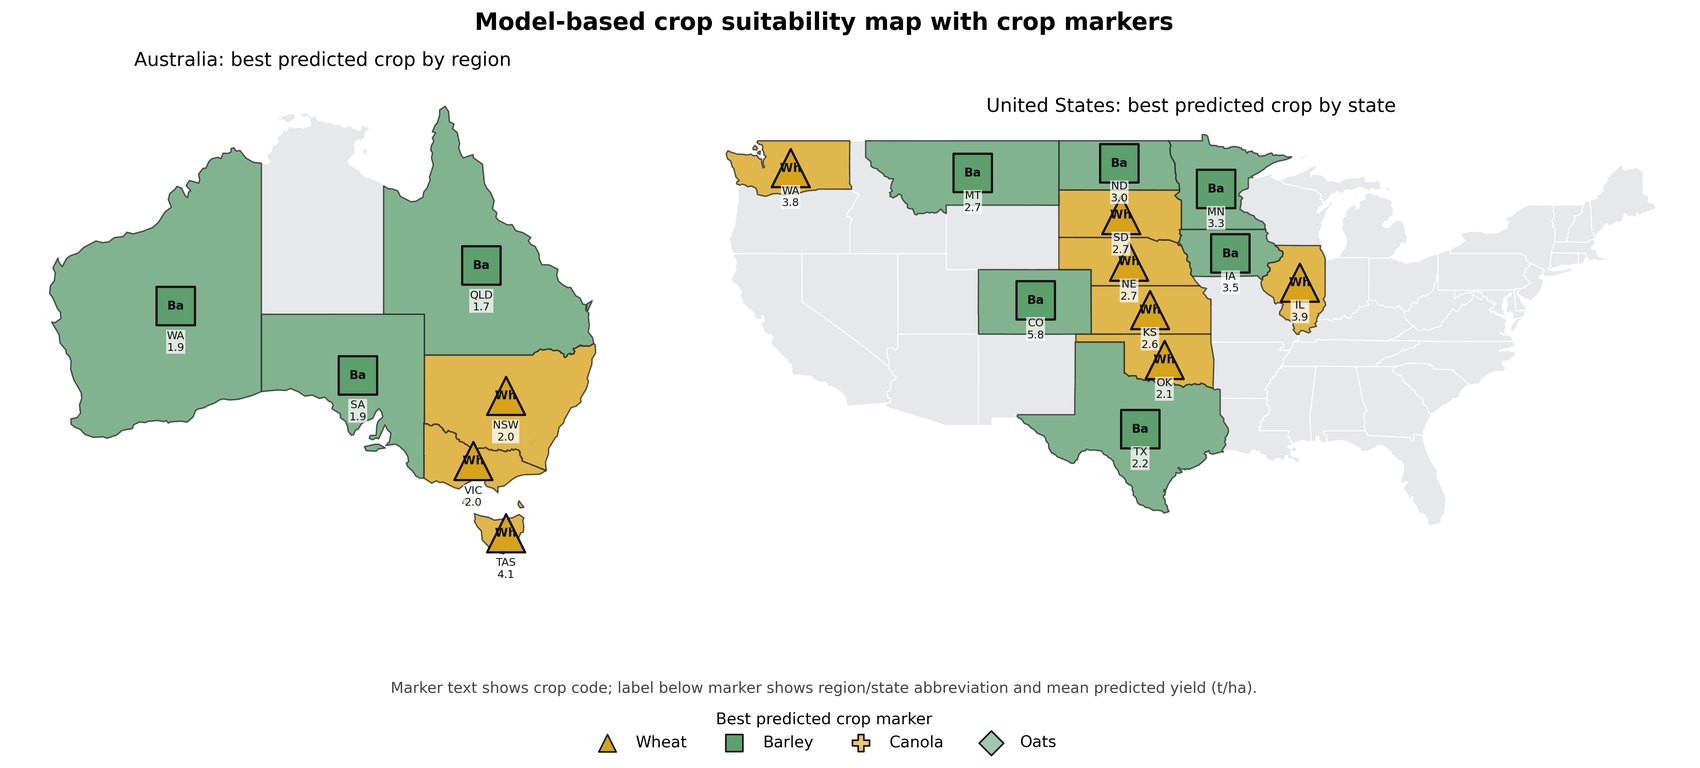
\includegraphics[width=\textwidth]{figures/main/fig07_crop_suitability_map.png}
\caption{Model-based crop suitability map. For each region, the map shows the crop with the highest predicted yield under the regional weather profile. Markers are decision-support signals, not prescriptive recommendations.}
\label{fig:suitability_map}
\end{figure}

\begin{figure}[H]
\centering
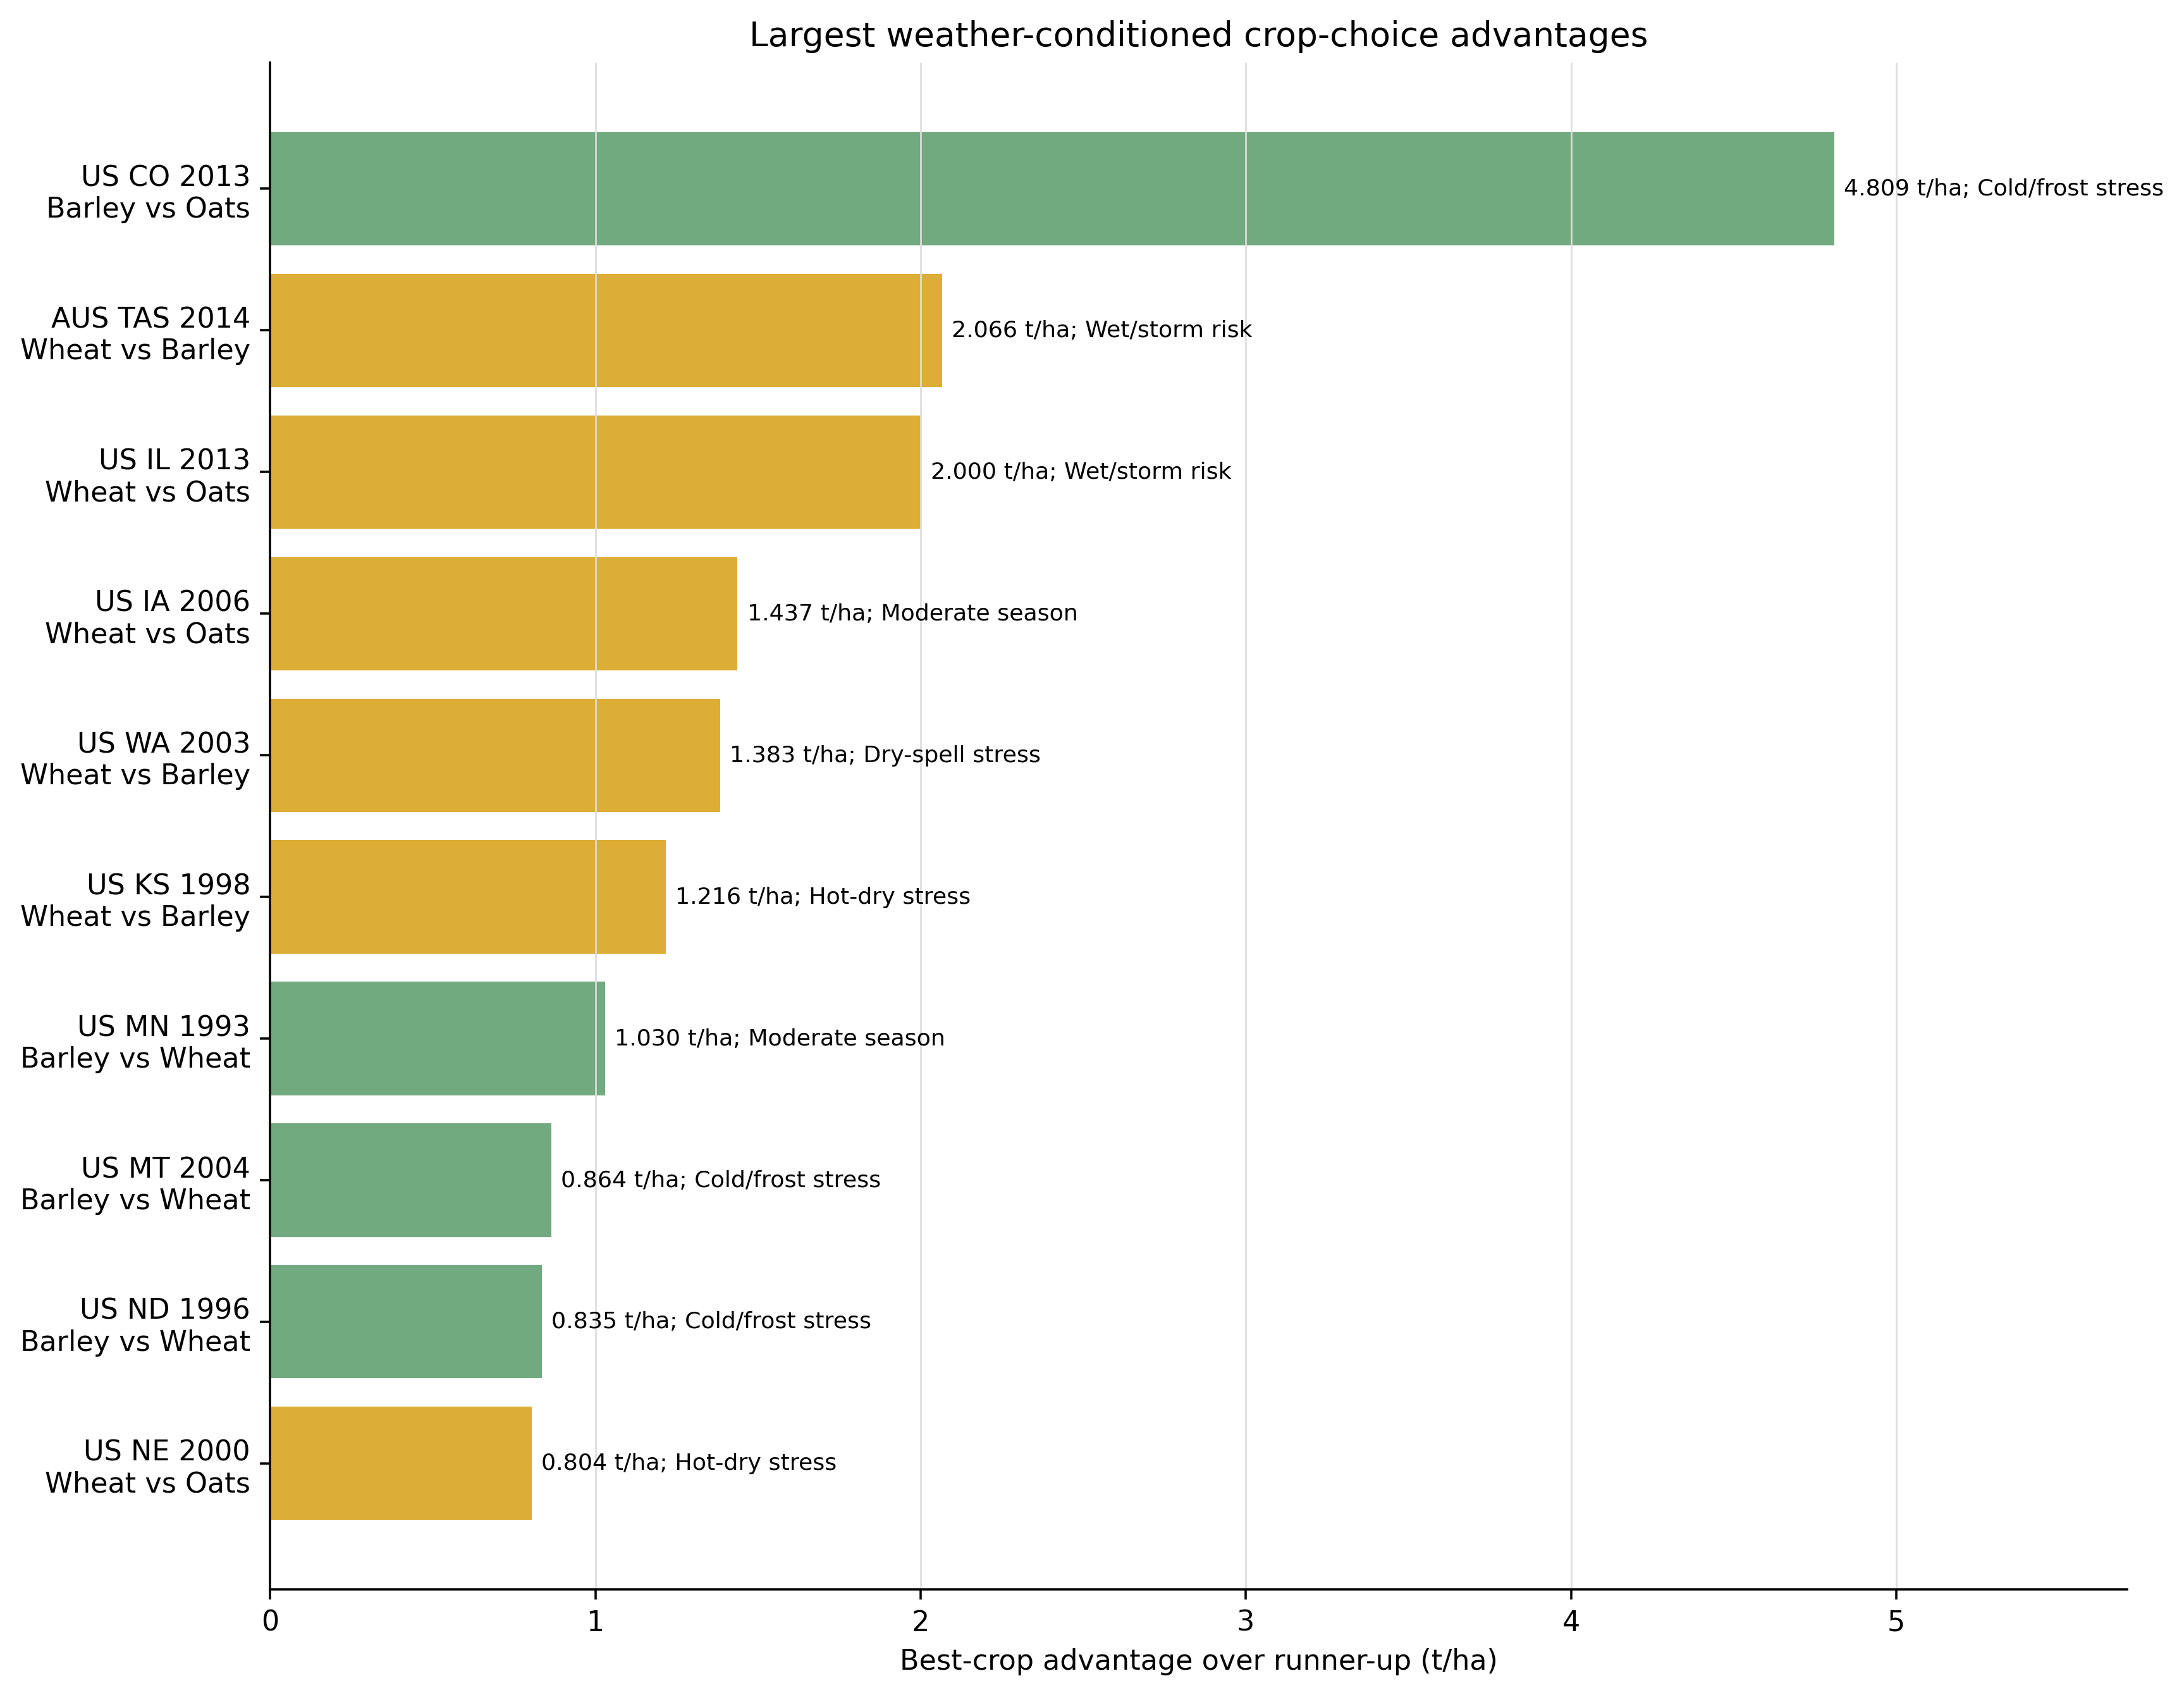
\includegraphics[width=\textwidth]{figures/main/fig21_weather_condition_crop_choice_advantage.png}
\caption{Weather-conditioned crop-choice advantage. The figure highlights region-year cases where the best predicted crop has the largest yield advantage over the runner-up crop under the same weather conditions.}
\label{fig:crop_choice_advantage}
\end{figure}

\FloatBarrier
\section{Discussion}
The results show that daily extreme-weather features are not only predictive, but also useful for explaining crop-region performance in operational terms. This supports the broader direction of multi-source and interpretable crop-yield modeling, where weather, soil, and environmental context are used to move from prediction toward actionable agricultural information \citep{Meghraoui2024DLReview,Lu2024MultiSourceDL,Mohan2025AIXAI}. The framework identifies where yield change is concentrated, which weather indicators distinguish favorable and unfavorable years, and which crops are predicted to be more suitable under the same region-year weather profile.

The crop-choice analysis should be interpreted as a screening layer rather than a direct prescription. It can help identify candidate crops or crop-region combinations for closer agronomic evaluation, but it does not replace local knowledge about irrigation, market demand, cultivar choice, disease risk, input costs, or management constraints. Its bootstrap intervals measure stability under resampling of the model-training frame, not full agronomic or economic uncertainty. This caution is especially important because yield models can degrade when moved across time, geography, or data domains \citep{Morales2023PastFuture,Joshi2024TransferLearning}.

\section{Limitations and Future Work}
This analysis is predictive and associative, not causal. The May--October growing season is a harmonized proxy and does not capture crop-specific planting, dormancy, harvest, or pre-harvest windows. Region-level data cannot fully represent within-region farm management, irrigation, cultivar, fertilizer, disease, or local soil variation. Weather products also differ across countries, with Australia and the United States relying on different source products. Future work should add crop-specific calendars, finer spatial resolution, management variables where available, and uncertainty intervals for crop-choice rankings. Remote sensing and UAV-based data streams are also promising extensions for improving spatial detail beyond the current tabular weather-soil frame \citep{Yuan2024UAVReview,Joshi2024TransferLearning}.

\section{Conclusion}
This study presents an interpretable daily extreme-weather framework for crop-yield prediction and crop-region suitability analysis. The main combined Australia and U.S. overlap-crop crop-region-year plus extreme-weather model, with the learning algorithm selected on the validation period and soil variables excluded, achieved competitive held-out predictive performance, although the previous-year yield baseline slightly outperformed it on the final test set. The post-model analysis translated predictions into crop-specific and region-specific planning signals by identifying yield gains and losses, weather signatures of high-yield years, and weather-conditioned crop-choice advantages. These outputs make the approach more useful for agricultural planning than a conventional yield-prediction leaderboard alone.

\begin{thebibliography}{30}

\bibitem{ABARES2026CropReport}
Australian Bureau of Agricultural and Resource Economics and Sciences.
\newblock \href{https://www.agriculture.gov.au/abares/research-topics/agricultural-outlook/australian-crop-report}{Australian Crop Report}.
\newblock 2026.

\bibitem{SILOClimate}
Queensland Government.
\newblock \href{https://www.longpaddock.qld.gov.au/silo/}{SILO: Australian climate data from 1889 to yesterday}.
\newblock 2026.

\bibitem{USDANASSQuickStats}
USDA National Agricultural Statistics Service.
\newblock \href{https://www.nass.usda.gov/Quick_Stats/}{Quick Stats Database}.
\newblock 2026.

\bibitem{USDANASSDeveloper}
USDA National Agricultural Statistics Service.
\newblock \href{https://www.nass.usda.gov/developer/}{Quick Stats API Developer Documentation}.
\newblock 2026.

\bibitem{NASAPOWERDaily}
NASA POWER Project.
\newblock \href{https://power.larc.nasa.gov/docs/services/api/temporal/daily/}{Daily API Documentation}.
\newblock 2026.

\bibitem{NASAPOWERParameters}
NASA POWER Project.
\newblock \href{https://power.larc.nasa.gov/docs/tutorials/parameters/}{Parameter Dictionary}.
\newblock 2026.

\bibitem{vanKlompenburg2020CropYieldReview}
T. van Klompenburg, A. Kassahun, and C. Catal.
\newblock Crop yield prediction using machine learning: A systematic literature review.
\newblock \emph{Computers and Electronics in Agriculture}, 177:105709, 2020.
\newblock \href{https://doi.org/10.1016/j.compag.2020.105709}{doi: 10.1016/j.compag.2020.105709}.

\bibitem{Paudel2021LargeScaleForecasting}
D. Paudel and others.
\newblock Machine learning for large-scale crop yield forecasting.
\newblock \emph{Agricultural Systems}, 187:103016, 2021.
\newblock \href{https://doi.org/10.1016/j.agsy.2020.103016}{doi: 10.1016/j.agsy.2020.103016}.

\bibitem{Saadio2022WestAfrica}
L. S. Cedric, H. W. Y. Adoni, R. Aworka, and others.
\newblock Crops yield prediction based on machine learning models: Case of West African countries.
\newblock \emph{Smart Agricultural Technology}, 2:100049, 2022.
\newblock \href{https://doi.org/10.1016/j.atech.2022.100049}{doi: 10.1016/j.atech.2022.100049}.

\bibitem{Sajid2022CountyScale}
S. S. Sajid, M. Shahhosseini, I. Huber, G. Hu, and S. V. Archontoulis.
\newblock County-scale crop yield prediction by integrating crop simulation with machine learning models.
\newblock \emph{Frontiers in Plant Science}, 13:1000224, 2022.
\newblock \href{https://doi.org/10.3389/fpls.2022.1000224}{doi: 10.3389/fpls.2022.1000224}.

\bibitem{Iniyan2023Techniques}
S. Iniyan, V. Akhil Varma, and Ch. Teja Naidu.
\newblock Crop yield prediction using machine learning techniques.
\newblock \emph{Advances in Engineering Software}, 175:103326, 2023.
\newblock \href{https://doi.org/10.1016/j.advengsoft.2022.103326}{doi: 10.1016/j.advengsoft.2022.103326}.

\bibitem{Panigrahi2023Comparative}
B. Panigrahi, K. C. R. Kathala, and M. Sujatha.
\newblock A machine learning-based comparative approach to predict the crop yield using supervised learning with regression models.
\newblock \emph{Procedia Computer Science}, 218:2684--2693, 2023.
\newblock \href{https://doi.org/10.1016/j.procs.2023.01.241}{doi: 10.1016/j.procs.2023.01.241}.

\bibitem{Jhajharia2023MLDL}
K. Jhajharia, P. Mathur, S. Jain, and S. Nijhawan.
\newblock Crop yield prediction using machine learning and deep learning techniques.
\newblock \emph{Procedia Computer Science}, 218:406--417, 2023.
\newblock \href{https://doi.org/10.1016/j.procs.2023.01.023}{doi: 10.1016/j.procs.2023.01.023}.

\bibitem{Morales2023PastFuture}
A. Morales and F. J. Villalobos.
\newblock Using machine learning for crop yield prediction in the past or the future.
\newblock \emph{Frontiers in Plant Science}, 14:1128388, 2023.
\newblock \href{https://doi.org/10.3389/fpls.2023.1128388}{doi: 10.3389/fpls.2023.1128388}.

\bibitem{Hu2023ExplainableYield}
T. Hu, K. Zhao, Y. Zhou, Y. Liu, G. Bohrer, J. Martin, Y. Li, and X. Zhang.
\newblock Crop yield prediction via explainable AI and interpretable machine learning: Dangers of black box models for evaluating climate change impacts on crop yield.
\newblock \emph{Agricultural and Forest Meteorology}, 336:109458, 2023.
\newblock \href{https://doi.org/10.1016/j.agrformet.2023.109458}{doi: 10.1016/j.agrformet.2023.109458}.

\bibitem{Schlenker2009NonlinearTemperature}
W. Schlenker and M. J. Roberts.
\newblock Nonlinear temperature effects indicate severe damages to U.S. crop yields under climate change.
\newblock \emph{Proceedings of the National Academy of Sciences}, 106(37):15594--15598, 2009.
\newblock \href{https://doi.org/10.1073/pnas.0906865106}{doi: 10.1073/pnas.0906865106}.

\bibitem{Lobell2011ClimateTrends}
D. B. Lobell, W. Schlenker, and J. Costa-Roberts.
\newblock Climate trends and global crop production since 1980.
\newblock \emph{Science}, 333(6042):616--620, 2011.
\newblock \href{https://doi.org/10.1126/science.1204531}{doi: 10.1126/science.1204531}.

\bibitem{Matiu2017TemperatureDrought}
M. Matiu, D. P. Ankerst, and A. Menzel.
\newblock Interactions between temperature and drought in global and regional crop yield variability during 1961--2014.
\newblock \emph{PLOS ONE}, 12(5):e0178339, 2017.
\newblock \href{https://doi.org/10.1371/journal.pone.0178339}{doi: 10.1371/journal.pone.0178339}.

\bibitem{Tack2015WarmingWheat}
J. Tack, A. Barkley, and L. L. Nalley.
\newblock Effect of warming temperatures on U.S. wheat yields.
\newblock \emph{Proceedings of the National Academy of Sciences}, 112(22):6931--6936, 2015.
\newblock \href{https://doi.org/10.1073/pnas.1415181112}{doi: 10.1073/pnas.1415181112}.

\bibitem{Pathak2023InputModalities}
D. Pathak, M. Miranda, F. Mena, C. Sanchez, P. Helber, B. Bischke, P. Habelitz, and others.
\newblock Predicting crop yield with machine learning: An extensive analysis of input modalities and models on a field and sub-field level.
\newblock \href{https://arxiv.org/abs/2308.08948}{arXiv:2308.08948}, 2023.

\bibitem{Bansal2023WinterWheatHeterogeneous}
Y. Bansal, D. Lillis, and M. T. Kechadi.
\newblock Winter wheat crop yield prediction on multiple heterogeneous datasets using machine learning.
\newblock \href{https://arxiv.org/abs/2306.11946}{arXiv:2306.11946}, 2023.

\bibitem{Dhaliwal2024SweetCorn}
D. S. Dhaliwal and M. M. Williams.
\newblock Sweet corn yield prediction using machine learning models and field-level data.
\newblock \emph{Precision Agriculture}, 25(1):51--64, 2024.
\newblock \href{https://doi.org/10.1007/s11119-023-10057-1}{doi: 10.1007/s11119-023-10057-1}.

\bibitem{Meghraoui2024DLReview}
K. Meghraoui, I. Sebari, J. Pilz, K. Ait El Kadi, and S. Bensiali.
\newblock Applied deep learning-based crop yield prediction: A systematic analysis of current developments and potential challenges.
\newblock \emph{Technologies}, 12(4):43, 2024.
\newblock \href{https://doi.org/10.3390/technologies12040043}{doi: 10.3390/technologies12040043}.

\bibitem{Mahesh2024Gradient}
P. Mahesh and R. Soundrapandiyan.
\newblock Yield prediction for crops by gradient-based algorithms.
\newblock \emph{PLOS ONE}, 19(8):e0291928, 2024.
\newblock \href{https://doi.org/10.1371/journal.pone.0291928}{doi: 10.1371/journal.pone.0291928}.

\bibitem{Jabed2024Comprehensive}
M. A. Jabed and M. A. A. Murad.
\newblock Crop yield prediction in agriculture: A comprehensive review of machine learning and deep learning approaches, with insights for future research and sustainability.
\newblock \emph{Heliyon}, 10(24):e40836, 2024.
\newblock \href{https://doi.org/10.1016/j.heliyon.2024.e40836}{doi: 10.1016/j.heliyon.2024.e40836}.

\bibitem{Lu2024MultiSourceDL}
J. Lu, J. Li, H. Fu, X. Tang, Z. Liu, H. Chen, Y. Sun, and X. Ning.
\newblock Deep learning for multi-source data-driven crop yield prediction in Northeast China.
\newblock \emph{Agriculture}, 14(6):794, 2024.
\newblock \href{https://doi.org/10.3390/agriculture14060794}{doi: 10.3390/agriculture14060794}.

\bibitem{Yuan2024UAVReview}
J. Yuan and others.
\newblock Grain crop yield prediction using machine learning based on UAV remote sensing: A systematic literature review.
\newblock \emph{Drones}, 8(10):559, 2024.
\newblock \href{https://doi.org/10.3390/drones8100559}{doi: 10.3390/drones8100559}.

\bibitem{Joshi2024TransferLearning}
A. Joshi, B. Pradhan, S. Chakraborty, R. Varatharajoo, S. Gite, and A. Alamri.
\newblock Deep-transfer-learning strategies for crop yield prediction using climate records and satellite image time-series data.
\newblock \emph{Remote Sensing}, 16(24):4804, 2024.
\newblock \href{https://doi.org/10.3390/rs16244804}{doi: 10.3390/rs16244804}.

\bibitem{Mohan2025AIXAI}
R. N. V. J. Mohan and others.
\newblock Next-gen agriculture: integrating AI and XAI for precision crop yield predictions.
\newblock \emph{Frontiers in Plant Science}, 2025.
\newblock \href{https://doi.org/10.3389/fpls.2024.1451607}{doi: 10.3389/fpls.2024.1451607}.

\bibitem{Ashfaq2025DeepAgroNet}
M. Ashfaq and others.
\newblock Predicting wheat yield using deep learning and multi-source environmental data.
\newblock \emph{Scientific Reports}, 2025.
\newblock \href{https://doi.org/10.1038/s41598-025-11780-7}{doi: 10.1038/s41598-025-11780-7}.

\end{thebibliography}

\end{document}
